%% ----------------------------------------------------------------------
%% START OF FILE
%% ----------------------------------------------------------------------

\documentclass[master,print]{xduthesis}
% \usepackage{showframe}
\usepackage{layout}
\usepackage{listings}  % don't forget [fragile] option after \begin{frame}
\lstset{language=C++, basicstyle=\ttfamily, numbers=none, xleftmargin=5pt, showstringspaces=false, frame=single} %keywordstyle=\color{red}
\usepackage{diagbox}
\usepackage{float}
\usepackage{enumitem}  % 带方括号的列举环境
\usepackage{etoolbox}  % 分支判断用

\newtoggle{blindreview}
\togglefalse{blindreview}
%\toggletrue{blindreview} %这行注释打开的话按盲审要求排(隐去作者信息)
\newtoggle{lookuprepeat}
\togglefalse{lookuprepeat}
%\toggletrue{lookuprepeat} %这行注释打开的话按查重要求排

\begin{document}
%\layout{}
%%%%%%%%%%%%%%%
%% 论文前置部分
%%%%%%%%%%%%%%%
\frontmatter

% 论文相关信息(封面)
\subjectcode{10701}
\subjectcode{10701}
\iftoggle{blindreview}{
    \studentid{~}
}{
    \studentid{1203121857}
}
\catelognumber{TP311.52}
\secretlevel{公开}

\ctitle{基于SSD的HDD缓存系统研究}
\etitle{A Research of HDD Caching System based on SSD}

\iftoggle{blindreview}{
    \cauthor{~}
    \eauthor{~}
    \csupervisor{~}
    \esupervisor{~}
}{
\cauthor{闫林}
\eauthor{Yan Lin}
\csupervisor{刘凯~教授}
\esupervisor{Prof. Liu Kai}
}

\cfirstdiscipline{计算机科学与技术}
\efirstdiscipline{Computer Science and Technology}
\cseconddiscipline{计算机技术}
\cdegreetype{工程硕士}
\cdate{2014年12月}
\edate{Dec 2014}

% 中英文摘要声明
%% ----------------------------------------------------------------------
%% START OF FILE
%% ----------------------------------------------------------------------

\begin{cabstract}

作为一种出现相对较晚的存储介质,固态硬盘(SSD)已经逐渐被部署到数据中心的存储阵列中。相比于机械硬盘(HDD),固态硬盘有着体积小、功耗低以及访问速度快的优势。但固态硬盘的高昂价格,使其难以在短时间内完全取代传统的机械硬盘。在许多存储中心,固态硬盘和机械硬盘是同时被部署的,且只有部分存储空间被用作存储。如果能将未使用的固态硬盘空间用作机械硬盘的缓存,系统IO性能将会得到明显的提升。

针对固态硬盘和机械硬盘同时存在但性能却没有得到充分发挥这一现状,本论文提出了一种基于SSD的HDD缓存系统解决方案:使用固态硬盘的存储空间作为机械硬盘的缓存,通过实现多种缓存管理算法,提升机械硬盘的IO性能。

基于数据局部性原理的缓存管理算法会在冷数据保持不变的前提下,将访问频繁的热数据在系统运行过程中由机械硬盘拷贝到固态硬盘,再次访问热数据的读写延迟将会很低。LRU、LFU以及一种论文提出的缓存页面替换算法将会被应用。这种新的页面替换算法综合考虑了缓存块的访问时间和访问频度因素,命中率更高且实现简单。用户利用配置工具,可指定某个固态硬盘卷用作缓存空间以及某个机械硬盘被缓存。实现的Windows存储卷过滤器驱动程序提供写穿和写回两种缓存运行模式。

论文实现的缓存系统不仅充分发挥了固态硬盘的性能,同时避免了存储系统向全固态硬盘迁移所带来的高昂成本。经测试,经固态硬盘缓存的机械硬盘将会有2-3倍的性能提升。

\end{cabstract}

\begin{ckeywords}
固态磁盘,机械硬盘,缓存系统,混合存储,数据局部性原理,缓存页替换算法
\end{ckeywords}

\begin{cthesistype}
应用基础研究类(或基础研究类)
\end{cthesistype}

%% ----------------------------------------------------------------------

\begin{eabstract}

Solid State Disk (SSD), as a new storage device, has been introduced into data centre because many of its advantages, such as compact size, low power consumption and high performance compared with Hard Disk Drive (HDD). But due to its relatively high price and low storage density, currently, SSD is mainly used in some high end storage subsystems. Actually, most of times, HDD and SSD exist in a system at the same time, and only a part of SSD's space is used. The IO performance of the storage system will be improved, if a software can configure part of the SSD as common storage while leaving unused part of SSD as a cache for HDD.

In order to solve this situation, this paper proposes a HDD-SSD hybrid storage solution using SSD as cache for HDD to improve HDD's IO performance.

Based on algorithm depending on data locality theory, the frequently accessed hot data on HDD will be copied to SSD, while leaving cold data on HDD. The latency will be very low to access hot data again. LRU, LFU and a new proposed cache page replacement algorithm are implemented to distinguish hot and cold data. This new proposed algorithm comprehensively considers time and frequency factors while its hit rate is high and it's easy to be implemented. Software is implemented as a Windows volume storage filter driver running in two modes: SSD as cache with write through strategy and SSD as cache with write back strategy. User can specify a SSD volume as cache's storage and a HDD volume as a cached device.

The proposed solution not only take performance advantage of SSD but also avoid costs to transfer all storage from HDD to SSD. With SSD cache, the I/O performance of HDD shows a 2-3x enhancement.

\end{eabstract}

\begin{ekeywords}
Cache, Data Locality, HDD, Hybrid Storage, Page Replacement Algorithm, SSD
\end{ekeywords}

\begin{ethesistype}
Applied Basic Research(or Basic Research)
\end{ethesistype}

%% ----------------------------------------------------------------------
%%% END OF FILE 
%% ----------------------------------------------------------------------

% 生成论文的封面、声明页、中英文摘要
\makecover

\iftoggle{lookuprepeat}{
}{
% 插图索引
\listoffigures
% 表格索引
\listoftables
% 其他列表
\chapter*{符号对照表}



\chapter*{缩略语对照表}


% 论文目录
\tableofcontents
}

%%%%%%%%%%%%%%%
%% 论文正文
%%%%%%%%%%%%%%%
\mainmatter

%% ----------------------------------------------------------------------
%% START OF FILE
%% ----------------------------------------------------------------------

\chapter{绪论}
\label{cha:introduction}

\section{研究背景}
\label{sec:background}

日新月异的计算机技术发展,带来了数据存储设备容量和CPU处理能力的大幅度提升。然而,磁盘系统的数据带宽以及I/O吞吐率的增长速度并未跟上CPU的步伐。与之而来的是CPU和传统磁盘系统的间愈发加大的速度差距(图\ref{fig:cpu-disk-diff})。

\begin{figure}[H]
\centering
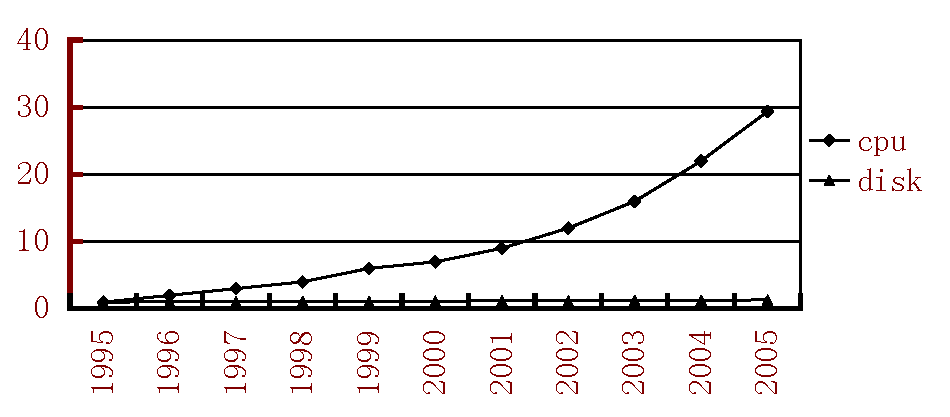
\includegraphics[width=0.7\linewidth]{./graph/cpu-disk-gap}
\caption{CPU与磁盘速度差异}
\label{fig:cpu-disk-diff}
\end{figure}

云端计算是继计算机系统从二十世纪80年代的大型计算机到“客户端-服务器”模式的又一次转变。与之而来的是对存储设备厂商对大数据(Big Data)越来越多的关注。大数据之所以会出现,是因为我们生活在一个拥有海量数据的信息社会中,21世纪人们与数据或信息交互比历史上的任何时期都要活跃。46亿全球移动电话用户中,有20亿人访问互联网,人们在畅游互联网的过程中,会自觉或不自觉的产生日志、访问历史和评论等信息,互联网上流动的交通量已经达到每年667艾字节。除了互联网,数据已经渗透到每一个行业和业务职能领域,并逐渐成为重要的生产因素。2011年5月全球知名咨询公司麦肯锡全球研究院发布了一份题为《大数据:创新、竞争和生产力的下一个新领域》的报告,报告指出了人们对于大数据的运用预示着新一波生产率增长和消费者盈余浪潮的到来。

大数据对存储系统的容量、速度及可靠性提出了非常高的要求,一些高性能的存储设备由此产生。固态硬盘(SSD)作为其中的佼佼者被引入传统的以机械硬盘(HDD)为主的存储系统。固态硬盘的读写性能远远高于传统的机械硬盘(表\ref{tab:ssd-speed-compare}),将固态硬盘引入存储系统中,将大大提高系统的性能。

\begin{table}[H]
\centering
\caption{HDD、DRAM和SSD的读写速度比较}
\begin{tabular}{|c|c|c|c|}
\hline  & Hard Disk & DRAM & SSD \\
\hline Read Access & 8.3ms & 60ns & 85ns \\
\hline Write Access & 9.1ms & 60ns & 4-10ms \\
\hline
\end{tabular}
\label{tab:ssd-speed-compare}
\end{table}

然而固态硬盘的价格仍然昂贵,虽然过去几年固态硬盘的价格一直快速下降,但下跌趋势正日益放缓,一系列问题导致固态硬盘和机械硬盘之间的价格差距不可能会很快消失。因此,固态硬盘不会在短时间内取代机械硬盘成为企业的主储存设备。固态硬盘的价格从2005年和2006年的3美元/GB跌至了2012年的0.67美元/GB,但与HDD的0.09美元/GB相比仍然相去甚远。根据固态硬盘历史价格的下降速度计算,到2020年它的价格约为0.15美元/GB,而届时机械硬盘的价格将会降至0.03美元/GB,对存储厂商来说机械硬盘仍然存在难以抗拒的价格优势。

综上,鉴于固态硬盘的价格较高且存储密度与机械硬盘差距较大,目前来讲,完全使用固态硬盘作为存储设备条件还不够成熟。虽然已有一些云计算存储中心部署了全固态硬盘的存储阵列,但是过高的成本令大多数使用者望而却步。为此,本文设计了一种既能保证成本在可接受的范围内,又能充分利用固态硬盘高IO性能的解决方案。

\section{相关研究工作}
\label{sec:related_works}

针对固态硬盘价格高、容量小、功耗低等特点,很多公司和研究者针对固态硬盘的使用场景,提出了基于固态硬盘的混合或分级存储解决方案。这些方案与全固态硬盘解决方案相比价格更能被接受。同时,相比于传统的使用DRAM作为缓冲区,基于NAND或NOR的固态硬盘有着功耗低(表\ref{tab:ssd-power-compare})、存储密度高以及可扩展性强的优势。

\begin{table}[H]
\centering
\caption{DRAM、Flash功耗比较}
\begin{tabular}{|c|c|c|c|}
\hline
\diagbox{介质}{功耗} & Density-Gb/cm2 & Active Power* & Idel Power* \\
\hline DDR2 DRAM & 0.7 & 878mW & 80mW \\
\hline NOR & 0.75 & 86mW & 16μW \\
\hline NAND & 1.42 & 28mW & 6μW \\
\hline
\end{tabular}
\\ * Power consumed for 1Gbit of memory
\label{tab:ssd-power-compare}
\end{table}

全球第六大企业软件公司EMC在2012年推出了VFCache解决方案。VFCache通过拦截不超过64KB大小的I/O请求(通常为随机操作)并将其缓存到PCIe闪存卡,从而达到加速访问的效果。由于不缓存应用程序的写操作,而是直接通过FCHBA卡写入后端SAN存储并等待其反馈成功信息,因此VFCache即便出现硬件故障也不会导致数据丢失。通过将固态硬盘引进存储阵列,EMC成为第一家涉足服务器PCIe闪存市场的主流厂商。

华为的云计算存储部门提出了解决方案SmartCache。SmartCache是一种将固态硬盘作为缓存资源的分层存储技术,是华为的一个动态数据缓存解决方案。SmartCache通过充当内存的扩展的方式,显著降低延迟并加快随机IO敏感性应用程序的执行速度,而无需以物理方式将数据移动到固态硬盘上。使用一个或多个固态硬盘作为磁盘阵列的缓存,称为SmartCache缓存池。统计HDD访问的热点数据,每隔一段时间移动到SSD的缓存池中。当热数据被访问时,就可以直接从缓存池中读取。该方案主要适用于IO请求中大部分为读,存在热点数据区域,且主要是位置随机的小请求的场景。

LSI作为一家知名的RAID适配器公司,推出了型号为LSI MegaRAID的SATA+SAS RAID控制卡。该RAID卡采用固态硬盘作为磁盘阵列的Cache存储热数据,从而有效提高读写性能,降低I/O时延,缩短RAID的访问和重建时间。结合LSI MegaRAID CacheCade Pro2.0软件,可以动态地将热数据从HDD阵列到SSD高速缓存中,操作完全透明,无需进行手动配置。

FC/SAS企业级闪存驱动器制造商STEC开源了Linux系统的EnhanceIO SSD缓存软件,能够加速任意类型的块存储设备——DAS/RAID/iSCSI/FC SAN。此外,EnhanceIO可以支持任意品牌型号的固态硬盘(包括SAS、SATA、PCIe和 Fibre Channel)作为缓存,同时针对STEC的产品有优化。缓存策略方面,EnhanceIO具备Read Cache(读缓存)、Write Back Cache(写回)和Write-through Cache(写通)三种模式,并能够在异常断电时阻止用户数据的丢失。

另一家SSD生产厂商,STEC的竞争对手Fusion-io也提出了自己的固态硬盘混合存储解决方案Fusion-io ioControl hybrid storage solution。与STEC不同的是,该解决方案针对云计算,能够很好的与虚拟机平台VMware Workstation以及Microsoft SQL Server clusters整合在一起,减少虚拟机和数据库查询的响应延迟。

\section{全文组织结构}
\label{sec:organization}

本文提出并实现了一种固态硬盘用作传统机械硬盘缓存的解决方案,在保证系统正确性和稳定性的前提下,考虑存储系统性能的提升。

全文组织结构如下。

第一章:绪论。论述当前云计算和大数据处理背景下对于存储系统性能的需求。对论文研究的意义以及国内外的相关研究工作加以简单描述。

第二章:相关技术简介。介绍与论文关系紧密的相关软硬件技术,包括SSD原理和特性、缓存系统的发展和评估、混合存储系统的原理和分类。

第三章:关键技术。介绍实现论文提出解决方案的实现中所涉及的关键技术,包括磁盘IO的捕获方式、缓存系统使用的页面替换算法、映射策略和索引结构以及缓存系统的两种回写策略。

第四章:缓存系统的实现细节。描述论文抽象出的Cache替换算法公共接口,并对每个接口的具体实现细节加以介绍。

第五章:实验和结果分析。从稳定性和性能两个角度对实现的系统进行测试,分析测试结果。于商业系统软件进行性能比较。

第六章:总结与展望。总结论文的研究成果和解决方案的贡献,展望进一步提升系统性能的改进方法。

%% ----------------------------------------------------------------------
%%% END OF FILE
%% ----------------------------------------------------------------------
%% ----------------------------------------------------------------------
%% START OF FILE
%% ----------------------------------------------------------------------

\chapter{背景技术简介}
\label{cha:related_work}

\section{存储介质简介}

\subsection{机械硬盘(HDD)}
机械硬盘\cite{hdd2009}(HDD,Hard Disk Driver)是个人计算机中一种应用最为广泛的非易失性的存储设备,使用覆盖有氧化铁的金属旋转盘片为存储介质。机械硬盘内部的物理结构分为磁盘、电动机、悬臂和主控芯片几部分。磁盘盘面以磁道、柱面和扇区的方式划分空间。电动机带动盘片旋转,副电动机带动悬臂上的磁头移动到碟片表面的某个位置。磁头悬浮在磁盘的正反两面上,磁盘旋转时磁头会在盘片表画出一个与磁盘同心的圆形轨道(称磁道或柱面)。此时,磁头内部的磁感线圈感应磁盘上的磁铁极性,通过时间间隔定位扇区,通过电流读取、写入数据内容到磁头所处的扇区。

通过磁化盘片表面上磁铁单元的极性,机械硬盘在平整的磁性表面上存储01比特数据。离磁性表面很近的读写磁头利用磁铁单元对电流的电感效应完成读写。盘片的两个存储面上各存在一个磁头负责读写,所有磁头的水平运用方向保持一致,磁头的移动方向由磁头控制器所负责。磁头只能沿盘片半径在水平方向上运动,结合电机带动盘片的高速旋转,磁头可以定位到盘片正反面上的任意位置进行记录数据的读写操作。

\begin{figure}[H]
\centering
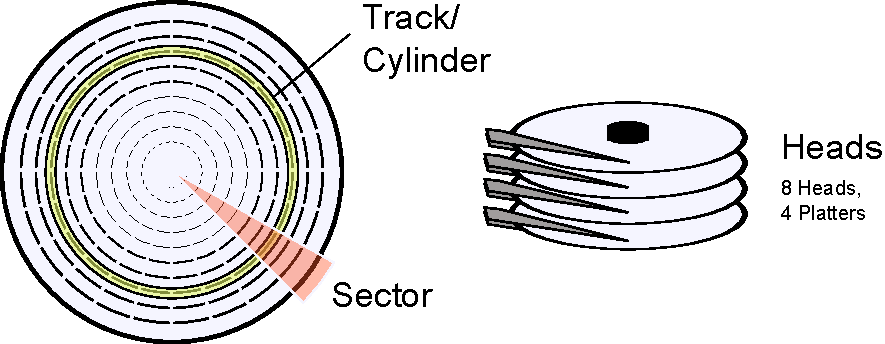
\includegraphics[width=0.6\linewidth]{./graph/hdd-struct}
\caption{机械硬盘结构}
\label{fig:hdd-struct}
\end{figure}

\begin{itemize}
\item 磁道
\\当磁头保持在某个位置上时,磁盘旋转,磁头会在磁盘表面画出一个与磁盘同心的圆圈,称该圆圈的轨迹叫做磁道(Track)。
\item 柱面
\\磁盘中通常存在一或多个盘片,竖直方向上的不同盘片、水平方向上同一半径的多个圆形磁道所组成的圆柱面,称为柱面(Cylinder)。
\item 扇区
\\每个圆形磁道按照角度又被等分为若干个弧段,每个弧段是硬盘上的一个扇区(Sector)。磁盘的首个扇区起名为引导扇区。
\end{itemize}

一般以RPM(每分钟的转动数)为单位描述机械硬盘盘片旋转速度,存在5400、7200、10000、15000几种规格。电机带动盘片转速越高,数据读写速率愈快,但噪音和发热量也上升明显。7200转属于最常见的磁盘转速。

机械硬盘内部的盘片、磁头机械结构决定了机械硬盘擅长于顺序读写,随机读写性能较差。

\subsection{固态硬盘(SSD)}
固态硬盘\cite{ssd2009}(SSD,Solid State Driver)作为一种存储设备,既可以基于永久性存储介质,如Flash闪存,也可以基于非永久性存储介质,如同步动态随机存取存储器(SDRAM)。设计固态硬盘的初衷是为了替代传统机械硬盘。固态硬盘内部已没有了像机械硬盘那样可以旋转的盘片结构,但是为了兼容人们对存储设备的命名习惯,固态存储器仍被称作硬盘。根据上面提到的所基于的两种存储介质,固态硬盘分为易失性和非易失性两类。

\subsubsection{基于易失性记忆体的固态硬盘}

使用易失性记忆体作为存储介质的固态硬盘,通常用于临时存放数据。易失性记忆体需要外界电力维持其内部的记忆功能,因此为了防止断电时的数据丢失,一般需要配合电池进行不间断供电。以SDRAM为代表的易失性存储介质,具有访问速度快(接近内存速度)、使用寿命长的优点。利用速度上的优点,软件程序可将需要访问的数据从机械硬盘转存到固态硬盘中,以此减少机械硬盘电机的启停延迟、磁头的寻道延迟对数据访问速度的影响。

此外,基于易失性记忆体的固态硬盘还可用于应急备份。这类固态硬盘一般会使用电池提供备用电力,即使遭遇意外停电,固态硬盘还可短暂利用电池电力,将数据转移到非易失存储设备。恢复电力后,再将数据从非易失存储设备转移过来。

\subsubsection{基于非易失性记忆体的固态硬盘}

基于非易失性记忆体的固态硬盘在外观上和机械硬盘已经没有什么区别。以NVRAM为代表的非易失性存储介质的数据存取速度,介于易失性介质SDRAM和机械硬盘之间。相比于易失性介质,非易失性介质数据一经写入,便无需额外电力以维持其存储能力,不必考虑断电的影响使其更具替代常规硬盘的潜力。

每块固态硬盘内部都会存在多个存储颗粒,每个存储颗粒中有非常多的存储单元储存数据。目前,市面上存在三种主流的制造固态硬盘存储单元的NVRAM颗粒,分別是多层式储存颗粒(MLC,Multi Level Cell)、单层式储存颗粒(SLC,Single Level Cell)和三层式储存颗粒(TLC,Triple Level Cell)。SLC、MLC和TLC三者的区别是存储颗粒内部单个存储单元所能存储的状态个数:SLC一种,MLC两种,TLC三种。这三者的读写速度几乎没有差别。TLC颗粒主要在企业级固态硬盘中使用,但是成本很高,使用MLC和TLC颗粒制造的固态硬盘的成本低,但是寿命较短。

由于存储颗粒内部每个存储单元的写入次数是有限的,存储颗粒的最大写入次数便是存储颗粒的使用寿命。固态硬盘控制器通常会把写操作平均分配到存储颗粒内部的每个存储单元上,再通过映射表的方式定位数据的实际存储位置。工业界使用P/E cycle这一参数标准衡量固态硬盘的使用寿命,一个P/E cycle代表了固态硬盘内所有的存储颗粒被写入一次。固态硬盘的P/E cycle参数体现了硬盘内部存储颗粒可写入次数的峰值,P/E cycle越大固态硬盘的使用寿命越长。

\begin{table}[htb]
\centering
\caption{SLC、MLC和TLC的寿命和价格比较}
\begin{tabular}{|c|c|c|c|}
\hline  & SLC NAND Flash & MLC NAND Flash & TLC NAND Flash \\
\hline P/E Cycles & 100,000 & 10,000 & 4,000 \\
\hline Cell type & 1bit/cell & 2bit/cell & 3bit/cell \\
\hline Price (USD/GB) & 5 & 1.4 & 1 \\
\hline
\end{tabular}
\label{tab:slc-mlc-tlc-compare}
\end{table}

从表\ref{tab:slc-mlc-tlc-compare}可以看出,存储颗的粒密度从SLC到TLC逐渐增大,而P/E cycle逐渐减少。SLC颗粒常被用于生产企业级的固态硬盘,而MLC颗粒和TLC颗粒则较多的出现于桌面计算机的固态硬盘中。虽然TLC颗粒的P/E cycle与SLC颗粒存在将近两个数量级的差距,但实际应用情况表明,使用TLC存储颗粒的固态硬盘完全可以满足桌面计算机的使用寿命要求。

尽管相比较于机械硬盘,固态硬盘有着如此多的优势,但使用非易失性颗粒的固态硬盘并非不存在缺点。当硬盘剩余空闲空间不多时,极可能出现严重影响写入性能的Write cliff现象。Write cliff现象出现在所有存储颗粒的空闲页都已经被初始化写入,新的写请求无法一次性得到足够的空闲页以完成写入操作的情况下。此时,固态硬盘控制器必须要擦除某些未写满的存储页面再进行写操作:控制器会将未写满存储页面的原有数据拷贝到临时空间,再进擦除;将原有数据与新数据进行合并,写入到擦除后的存储页面。拷贝原有数据到临时空间消耗的时间是Write cliff出现的主要原因。

为减少Write cliff对性能的影响,固态硬盘厂商特别加入了针对固态硬盘数据删除的TRIM指令。当需要删除文件时,可通过TRIM指令会告知固态硬盘被删除文件的位置,固态硬盘控制器会将对应的存储块标记为空闲状态。这样,就能在一定程度上保证总是存在空闲页,从而降低Write cliff现象的出现概率。TRIM指令的出现,很大程度上提升了固态硬盘的性能、延长了固态硬盘的寿命。但当空闲页面无法满足写请求时,仍然需要擦除未写满的存储页面。因此,TRIM命令只能推迟,但无法避免Write cliff现象的出现。

\subsection{机械硬盘与固态硬盘的比较}
固态硬盘出现的目的是替代传统的机械硬盘,但是机械硬盘相较于固态硬盘的某些优势使得固态硬盘不可能在短期内动摇机械硬盘的统治地位。两者之间的差别可从以下几个方面进行比较。

\subsubsection{安全性}
机械硬盘内部的盘片、电机等机械构造决定了在发生碰撞和震动时,磁头和盘片的接触往往会造成机械硬盘的损坏,从而导致数据的丢失。固态硬盘内部使用的缓存芯片几乎不受碰撞和震动的物理影响。

\subsubsection{性能}
无论是启动速度还是IO性能,固态硬盘都有着非常明显的优势。造成这种优势的主要原因是固态硬盘内部不是机械结构,不需要寻道以定位数据。传统的机械硬盘则需要在指令接受后开始寻道。因此固态硬盘在读写速度,尤其是随机读写上,较普通机械硬盘存在很大优势。

\subsubsection{价格}
2012年的统计数据表明,固态硬盘的价格是0.67美元/GB,传统的机械硬盘的价格是0.09美元/GB,固态硬盘价格是机械硬盘的7倍多。造成价格悬殊的主要因素是机械硬盘发展较早,技术相对成熟;固态硬盘制造工艺则有待提高。固态硬盘的高昂价格会让很多用户在购买前三思,他们更倾向于暂失固态硬盘的诸多优势而选择性价比更高的机械硬盘。

\subsubsection{容量}
海量数据时代的到来和用户对更高品质交互体验的追求,带来了日益增长的数据存储空间需求。大容量固态硬盘不仅非常稀少且价格昂贵,主流的固态硬盘一般都为128GB、256GB或512GB的存储空间。实际情况是,1TB的机械硬盘都已难以满足桌面电脑的需求,更不用说数据量巨大的企业级用户。

\subsubsection{耗电量}
机械硬盘使用电机驱动盘片旋转和磁头移动,耗电量约为固态硬盘的3倍多。对于移动设备来讲,耗电量的多少是衡量电池所能支持待机时间的关键。同样的,在存在上百个磁盘阵列的数据中心部署固态硬盘,可以节约大量电能,从而减少电费支出。但基于易失性存储器的固态硬盘需要不间断供电,否则可能会导致数据丢失。

\subsubsection{重量和形状}
由于不存在机械硬件的磁盘、电机等部件,固态硬盘的平均重量仅仅有70-85克,而机械硬盘则可达到650-800克,这一优势可使便携的移动设备同时搭载几个固态硬盘成为可能。同时,完全半导体化的固态硬盘内部结构,使其在物理上无样式、结构的限制,可根据实际需求改变固态硬盘的接口、形状。

\subsubsection{工作温度}
固态硬盘本身的功耗就不高,所以其在工作过程中产热也相对较低。而机械硬盘每分钟5000转以上的转速,盘片和空气的摩擦以及不同机械部件之间的摩擦所产生的热量远高于固态硬盘,温度太高很容易使机械硬盘的脱离正常工作状态。固态硬盘不但本身产生的热量少,而且能够工作在更宽泛的温度范围内。

\subsubsection{噪音}
得益于使用闪存芯片存储,固态硬盘不会产生噪音。而机械硬盘运行时则会产生一定的噪音。尤其是存储中心大规模的磁盘阵列所产生的巨大噪音,更是需要设立专门的机房进行存放。

\section{存储系统缓存技术}
\label{sec:storage_cache_tech}

尽管自二十世纪九十年代以来,计算机硬件技术的发展带来了磁盘存储密度每半年到一年一倍的提升,但没有相应的技术能够以同样的速度缩短存储介质的访问时间。缓存技术\cite{cache2011}作为一种减少IO子系统的响应时间、增加系统吞吐量的解决方案,已被广泛应用于存储子系统中。

\subsection{缓存的特点}
保存了主存储器中少部分数据复制品的缓存,其访问速度远高于主存储器。如果仅使用缓存中的数据,就可以满足某次主存的访问请求,则称缓存命中了一次。

由于缓存中保存的是主存储器中的部分数据,因此会出现找不到所需数据而无法命中的情况,此时则需要访问主存储器才能获得数据。如果这种情况发生的比例超过一定数值,缓存对系统性能的提升就无法得到保证。不命中情况下获得的主存储器数据被用来更新缓存内的数据内容,以提升下次访问在缓存中命中的概率。由于被频繁访问的热数据并非一成不变,因此需要缓存页面替换算法不断更新缓存内的数据,才能保证缓存中的数据是被再次访问的概率最大,命中率才能有保证。

\subsection{缓存的工作原理}
为形象说明缓存系统的工作原理,本小节以CPU访问内存中的数据为例进行说明。绝大多数CPU中都集成了一或多级的高速缓存以减少直接访问内存次数。

CPU执行过程中需要内存中的某个数据时,首先会从高速缓存中查找,如果能够找到,则无需访问内存即可进行处理,几乎没有响应延迟;如果没有找到,就只能从延迟较高的内存中读取后再送给CPU进行处理,同时,将获得的数据块调入高速缓存中。更新缓存中的数据一定程度上可以增加数据在缓存中进行的概率,减少内存的访问。正是这一机制使大多数CPU的高速缓存命中率可达到90\%左右,只有10\%的访问操作需要真正读取内存。减少了需要CPU直接访问内存的次数,也就使得CPU几乎无需等待,便可获得所需数据。一般来说,CPU需要数据时总是先查缓存、后访内存。

\subsection{缓存数据替换算法}
缓存系统运行过程中,需要对存储设备上的数据按照请求的频率进行冷热程度的划分。性能较高的存储设备储存经常访问的热数据,存储在性能较低的设备储存不经常访问的冷数据,以达到区分对待冷热数据的效果。缓存数据替换算法在缓存系统运行过程中,通过识别出的冷热数据,不断移动和更新缓存中数据,尽可能保证热数据存储在性能较高的存储设备,以达到提升缓存命中率和系统性能的双重目的。所以,从本质上讲,缓存数据替换算法,就是数据的热度识别和存储空间管理算法。

从缓存提升系统性能的原理不难得出,区分冷热数据的准确程度直接影响了缓存系统的IO性能。学术上已经有很多关于区分冷热数据的算法研究成果。根据缓存空间组织的粒度,缓存数据替换算法可以分为两类,不同类型算法有不同的识别准确程度和计算复杂度。下面会逐一进行介绍。

\subsubsection{数据块级}

数据块是最小的数据空间划分单位,通过数据块识别冷热数据需要将主存储空间和缓存空间按照相同大小的数据块进行划分。将数据块看作是统计冷热程度的最小单位,通过统计每个数据块的访问计数,将标记访问计数大的数据块为热数据块。在设计固态硬盘的读写逻辑时,数据块的热点识别用于实现损耗平衡:通过一定的映射策略,将写操作平均分配给所有的存储块。

数据块级的冷热数据识别的优势在于,它可以在文件系统无关的存储层面精确地定位出所有的热数据块,同时又不必在考虑例如存储空间组织结构、文件系统等宏观的信息,从而简化了识别冷热数据的计算过程,保证了系统性能受计算复杂度的影响尽可能小。

\subsubsection{文件级}

文件级别的冷热数据划分\cite{linlin2011}是另一种常用到的判定方法。这种以文件作为最小热度统计单位的方法,为每个文件开辟了专用于存储访问计数值的元数据区域。所有文件访问操作都会改变元数据区域中的计数值。文件级别的冷热数据划分可以从文件类型、文件大小、同时打开文件的进程数目等多种宏观层面指标进行综合评估,提升判别的准确程度。

相比于数据块级别,文件级判别对统计数据存储空间的使用更为节约,进而降低了缓存系统的额外空间消耗。而且还可以将随机性因素加入文件访问的识别过程,更好的区分冷热数据文件。

\subsection{缓存系统存在的目的}
缓存系统的存在通常是为了达到三个目标:
\begin{enumerate}
\item 减少交互的通讯量:缓存数据能最小化进程和网络间传输的数据量。
\item 降低系统的处理量:记录处理结果,避免数据的重复处理。
\item 降低主存储器的访问次数:如操作系统内核在内存中缓存的机械硬盘数据。
\end{enumerate}

在评估一个缓存系统的好坏时,一般会从性能、稳定性和可用性三个方面进行:
\begin{enumerate}
\item 性能:定量分析访存请求在缓存中的命中率和带来的延迟缩短。
\item 稳定性:缓存算法的时空复杂度是否稳定性,对于意外情况(如掉电),能否保证数据完整。
\item 可用性:缓存系统对应用是透明的,应用感受到的,仅仅是飞快的响应速度和良好的可用性。
\end{enumerate}

\section{混合存储系统}
\label{sec:hybrid_storage}

只要数据处理速度和存储介质访问速度、不同类型存储介质的访问速度之间仍然存在大的差距,学术和工业界就不会停止研究、探索和利用不同速度存储器件,搭建混合存储系统\cite{zhuqing2013hybrid},以提高低性能介质的性能、可靠性等指标。经过近二十年的研究,科学家和工程师们已经取得了众多的研究成果。

\subsection{基于DRAM与机械硬盘的混合存储}

使用DRAM为机械硬盘缓存数据\cite{sdramcache2002},毫无疑问,是提高机械硬盘性能的重要手段之一。几乎所有操作系统在设计磁盘驱动程序时,都会优先考虑使用DRAM缓存机械硬盘的数据。硬盘制造商在制造硬盘时,同样会在硬盘控制器中加入8-16MB的DRAM芯片。利用数据的空间局部性原理,硬盘控制器在处理IO请求时读取的数据量会略大于请求的数据量,并在DRAM进行缓存。对于软件来说,处于硬盘控制器中的DRAM缓存是透明的,磁盘驱动程序不必关心控制器如何管理缓存。

由于DRAM的易失性限制,通常只使用DRAM作为读缓存提高机械硬盘的性能,因而对写性能几乎没有提高效果。如果也缓存写操作,为了避免写入机械硬盘的脏数据由于掉电而丢失,磁盘控制器或是驱动程序就必须将脏数据持续的从DRAM写回到机械硬盘,以降低数据丢失的风险。因此,使用DRAM缓存面临着数据可靠性和读写性能间的两难选择,缓存越大性能提升越明显,停留在缓存中的脏数据丢失的可能性也就越大。基于以上原因的考虑,任何缓存系统都会限制缓存中脏数据的停留时间和所占比例。

\subsection{基于NVRAM与机械硬盘的混合存储}

NVRAM非易失性的据存储数优势,使得利用NVRAM作缓存提升存储系统写性能也成为可能。常用的一种策略是整合NVRAM缓存与DRAM缓存\cite{nvramcache2013},遇到写操作时,同步写入数据到两种缓存。NVRAM的非易失性保证了数据的可靠性,DRAM的高性能保证了性能的提升比例。只有意外掉电情况发生时,NVRAM内的备份数据才会被启用,并重新写回到机械硬盘;另一种策略是合并DRAM和NVRAM为一个的存储空间,缓存块存储于哪种类型的存储器由算法决定,涉及写操作的脏数据块必须存放于NVRAM。

NVRAM的小容量特性,使得其对机械硬盘性能提升的贡献非常有限。虽然近5年来的技术革新带来了NVRAM容量的不断提高,但是相比于增长更为迅速的机械硬盘存储空间,加上海量数据访问时呈现出的一次性的访问特征,使得基于NVRAM的机械硬盘缓存命中率难以有大的提升,系统读写性能的提升效果也非常有限。

\subsection{高低转速磁盘的混合存储}

机械硬盘中磁盘盘片的物理转速直接决定了处理读写请求的速度。因此,混合不同接口、不同转速的机械硬盘架设混合存储系统,曾一度是20世纪90年代存储界研究的热点之一。

高低转速磁盘混合存储的原理是:根据数据的访问热度、保留时间、优先级等指标,将访问频繁的热数据存储在转速为10000-15000 RPM的高性能SCSI机械硬盘中;访问热度低的冷数据则被存储在转速为5400-7200 RPM的性能普通的IDE(或SATA)机械硬盘中。但由于机械硬盘内部物理器件的极限限制,不同转速盘片所带来的性能差距并不显著。而且,随着固态盘的出现,这种混存系统近年来已很少被使用。

\subsection{基于固态硬盘和机械硬盘的混合存储}

固态硬盘和机械硬盘之间性能的良好互补性,以及近几年来高寿命、高密度的固态硬盘存储设备生产技术的日渐成熟,都为设计基于固态硬盘和机械硬盘的混合存储系统提供了崭新的契机。这种混合存储解决方案已成为海量数据存储技术中的一个新的发展方向,并已经成为了学术界的研究热点。理论研究的发展同时带来了企业存储解决方案如雨后春笋般的提出:微软,LSI,Intel,EMC,IBM, FusionIO等企业都已经或即将推出基于固态硬盘的混合存储解决方案。

\section{缓存算法评估}
\label{sec:cache_evaluation}

大多数学术论文在评估某种缓存替换算法的优劣时,都是只评估替换算法带来的缓存命中率。为了提高论文的说服力,有的还会给出该算法应用于某种环境所带来的性能提升比例。当工程师为混存系统挑选一种合适的缓存算法时,这些数据的参考价值都很有限,且不存在一种通用的评估方法。
下面介绍一种本论文提出并使用的缓存算法的评估模型,该模型既可以用于评估缓存算法给系统可能带来的性能提升,又可以为缓存系统工程师设计系统起到指导作用。

给出评估方法之前,式\ref{equ:cache_evaluation_syms}列出了推理中用到的数学符号。
\begin{equation}
\begin{split}
\\&T_1=\mbox{无缓存时,单个读/写请求处理时间}
\\&T_2=\mbox{有缓存且缓存命中时,单个读/写请求的处理时间}
\\&T_3=\mbox{有缓存但缓存时,单个读/写请求的处理时间}
\\&N=\mbox{读写请求总数量}
\\&R=\mbox{缓存命中率},R\in\lbrack0,1)
\\&T_q=\mbox{查询一个读/写请求在缓存池中是否命中的时长}
\\&T_c=\mbox{从缓存池拷贝或向缓存池写入完成一个读/写请求所需数据的时长}
\\&T_u=\mbox{使用单个未命中的读/写请求数据,更新缓存池所需时间}
\end{split}
\label{equ:cache_evaluation_syms}
\end{equation}

评估缓存对于系统IO性能的提升,可以用有、无缓存前提下,读写请求花费总时长的变化比例来表示。

\begin{equation}
\begin{split}
\mbox{性能提升比例}&=\frac{\mbox{无缓存条件下完成所有读写请求的总时长}}{\mbox{存在缓存时完成所有读写请求的总时长}}
\\&=\frac{NT_1}{NRT_2+N(1-R)T_3}
\\&=\frac{T_1}{RT_2+T_3-RT_3}
\\&=\frac{T_1}{T_3-(T_3-T_2)R}
\end{split}
\label{equ:cache_evaluation_enhance1}
\end{equation}

系统不存在缓存时,一个读/写请求所需的时间($T_1$)等同于该读/写请求直接应用于存储介质上所需的时间。

系统存在缓存且请求命中时,缓存系统利用缓存中数据即可完成读/写请求。这时,一个读/写请求所需的时间($T_2$)等同于查询缓存池所需时间($T_q$)加上从缓存池拷贝或向缓存池写入完成一个读/写请求所需数据的时间($T_c$)。
\begin{equation}
T_2=T_c+T_q
\end{equation}

系统存在缓存但未命中时,为了完成请求需要应用请求于存储介质,再使用获得的数据(读请求)或请求中包含的数据(写请求)更新缓存池。这时,一个读/写请求所需的时间($T_3$)等同于查询缓存池所需时间($T_q$),加上应用读/写请求于存储介质所需时间($T_1$),再加上使用新数据更新缓存池所需的时间($T_u$)。
\begin{equation}
T_3=T_q+T_1+T_u
\end{equation}

综上可以得出$T_2$与$T_3$的关系,同时,$T_3$也可以用$T_2$来表示(式\ref{equ:cache_evaluation_t2t3})。

\begin{equation}
T_3-T_2=T_1+T_u-T_c
\end{equation}
\begin{equation}
\label{equ:cache_evaluation_t2t3}
T_3=T_1+T_2+T_u-T_c
\end{equation}

最后,将式\ref{equ:cache_evaluation_t2t3}带入到提升比例计算公式\ref{equ:cache_evaluation_enhance1},得出最终的性能提升比例计算公式\ref{equ:cache_evaluation_enhance2}。

\begin{equation}
\begin{split}
\mbox{性能提升比例}&=\frac{T_1}{T_3-(T_3-T_2)R}
\\&=\frac{T_1}{(T_1+T_2+T_u-T_c)-(T_1+T_u-T_c)R}
\\&=\frac{T_1}{T_2+(T_1+T_u-T_c)(1-R)}
\\&=\frac{T_1}{T_q\textdownarrow+T_c+(T_1+T_u\textdownarrow-T_c)(1-R\textuparrow)}\textuparrow
\end{split}
\label{equ:cache_evaluation_enhance2}
\end{equation}

$T_1$取决于被缓存储介质的性能;$T_c$取决于缓存存储介质的性能。这两个值在硬件环境一定的情况下为定值。

提升缓存系统性能就是提高缓存系统为原系统带来的性能提升比例。式\ref{equ:cache_evaluation_enhance2}表明,可以从以下三个点着手:

\begin{enumerate}
\item
提高缓存池的查询速度,缩短查询时间$T_q$。
\item
提高缓存池的更新速度,缩短更新时间$T_u$。
\item
优化缓存算法,提高缓存命中率$R$。
\end{enumerate}

从工程经验的角度讲,上面提高缓存系统性能的三个着手点也是行得通的。

%% ----------------------------------------------------------------------
%%% END OF FILE
%% ----------------------------------------------------------------------
%% ----------------------------------------------------------------------
%% START OF FILE
%% ----------------------------------------------------------------------

\chapter{关键实现技术}
\label{cha:key_tech}

本章介绍实现混合存储系统用到的关键技术。从系统如何捕获程序对机械硬盘的读写操作为开始,介绍WDM驱动程序架构和IO捕获实现原理。接着介绍了缓存系统的核心逻辑,缓存页面替换算法,逐一说明论文所实现的三种页面替换算法的原理和实现方式。然后,说明了决定缓存系统缓存块映射方式的三种缓存映射策略。本论文实现的缓存系统使用了全相联映射,所用到的B+树索引数据结构也会在本章介绍。最后,给出缓存系统运行于写回和写穿模式时的脏缓存块回写策略。

\section{IO捕获}
\label{sec:capture_io}

缓存系统实现的第一步,是捕获上层应用程序对机械硬盘的读写操作。本论文在Windows操作系统平台实现缓存系统,以存储卷过滤器驱动程序的方式,实现了对机械硬盘的存储卷设备的IO捕获功能。为了更好描述驱动程序对捕获IO的方式,本节先会对Windows驱动程序开发模型(WDM)加以介绍,然后说明过滤器驱动程序组织结构以及在系统内核中所处的位置。下一章将会详细说明代码的实现细节。

\subsection{Windows驱动程序模型(WDM)}
Windows驱动程序模型(Windows Driver program Module, WDM)是一种针对使用Windows NT操作系统内核的Windows驱动程序的设计规范\cite{wdm2001}。这一规范定义了一整套的驱动程序开发所使用的函数接口、数据结构、组织关系和模块间的交互协议。

WDM模型按照面向对象的程序设计思想,将操作系统内核中的所有组件都划分为不同类型的设备对象(Device Object)和驱动对象(Driver Object)。设备对象既可以对应具体的硬件设备,如磁盘、键盘、显示器,也可以对应逻辑上存在的设备,如存储卷、虚拟光驱、Ramdisk。驱动对象对应了加载到内核中驱动程序,如显卡驱动程序、网卡驱动程序、鼠标驱动程序。一台计算机可以存在多个同种类型的硬件设备,这些设备只需要一个对应的驱动程序就可以驱动。也就是说,一个驱动程序可以管理多个同种类型的设备对象。

驱动对象的职责是管理设备对象,因此设备对象这种内核数据结构都由驱动对象所创建并注册。驱动对象可以在设备对象不存在时独立存在。没有驱动对象为硬件设备创建的设备对象,硬件设备也不可能正常运行。图\ref{fig:drv-to-dev}描述了这样一种从驱动到设备一对多的对象之间的关系。
\begin{figure}[!htb]
\centering
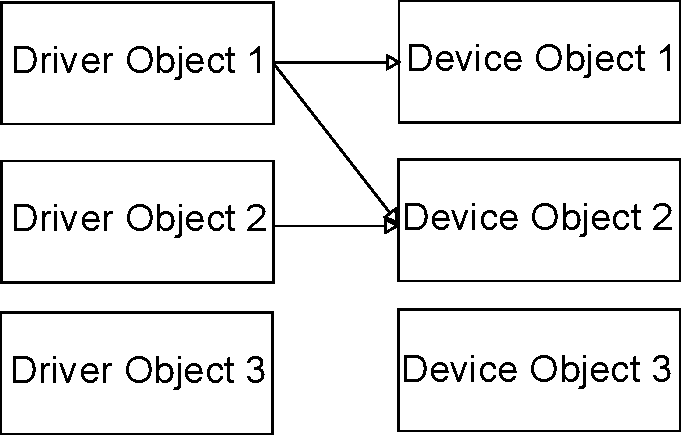
\includegraphics[width=0.6\linewidth]{./graph/drv-to-dev}
\caption{设备对象和驱动对象的对应关系}
\label{fig:drv-to-dev}
\end{figure}

从功能的角度讲,WDM驱动模型被分为三类:
\begin{enumerate}
\item
总线型驱动:驱动某种类型的计算机总线设备,为这种总线上挂载的每个设备提供独立的功能接口。检测和处理总线类型设备的加载和移除事件,负责总线上硬件的驱动程序注册、卸载和仲裁等管理工作。
\item
功能型驱动:驱动某种指定类型的硬件设备,通过和设备间的数据交互实现某一功能,并提供给上层应用程序访问硬件的API接口。如果设备挂载在某种数据总线上,还需要向总线驱动注册总线事件的回调函数。一般由硬件生产厂商提供,在大多数硬件环境下,一个功能型驱动会服务多个硬件设备。
\item
过滤器型驱动:过滤发送给某个设备或是某种类型的硬件总线的操作请求,对捕获到的IO请求进行选择性的处理。过滤器驱动程序对捕获到的请求的处理方式可以是任意的:直接传递给下一个设备对象、处理后再传递或是处理后返回并结束该IO请求。
\end{enumerate}

实践证明,鉴于WDM模型对于驱动程序模块化的组织和规范化的接口要求。使用WDM模型开发硬件驱动程序会使系统内核更加稳定,操作系统可以更高效地操纵硬件。更重要的是,不仅作为驱动程序与操作系统交互的标准接口,WDM还强调驱动程序应该采用模块化的体系架构和设计思想,从而简化调试过程中的错误定位过程。

\subsection{IRP和驱动程序堆栈}
IRP(I/O request package)是Windows内核中描述驱动程序模块之间交互协议的数据描述。上层应用程序通过调用操作系统提供的API函数,进行和设备或文件的交互工作。而API函数的实现中,则需调用IO管理器完成交互请求。IO管理器根据操作的类型将交互信息封装成相应的IRP请求,并发送给对应的设备对象。IRP最终会以调用参数的形式,传递给驱动内部不同类型的分发函数。处理结束后,IO管理器将包含分发函数返回结果的IRP进行解包,返回应用程序的所需信息。

驱动程序堆栈是从应用层API到硬件访问接口的一整套驱动程序。大多数情况下,一个硬件设备能够正常运转依靠的是多个驱动程序的协同工作,这些驱动程序创建的设备对象按消息处理的顺序层次化组合在了一起,构成了设备的驱动程序堆栈。IRP扮演了驱动程序堆栈中层与层之间消息传递的媒介:IRP通过每个设备所唯一对应的驱动程序堆栈,自上而下将用户操作传达至硬件设备;驱动程序将从硬件设备获得的数据存入IRP,自下而上返回给上层应用。

因此,捕获IO操作本质上是捕获驱动程序堆栈中IRP的操作。

\subsection{驱动程序分发函数}
设备对象接收到IRP后,将其作为参数传递给驱动程序的分发函数。驱动程序通过IRP内部保存的分发函数类型码(IRP\_MJ\_XXX)确定用于处理该IRP的分发函数。Windows系统定义了针对不同类型设备的一整套分发函数码。驱动程序要能正常运行,必须实现表\ref{tab:must-handled-major-function}中的所有分发函数。

\begin{table}[!htb]
\centering
\caption{驱动程序必须提供的分发函数}
\begin{tabular}{|ll|}
\hline IRP\_MJ\_PNP  & 识别、配置PnP设备,分配硬件资源。 \\
       IRP\_MJ\_POWER & 处理电源管理器发出的电源请求。 \\
       IRP\_MJ\_CREATE & 处理用户程序打开设备对象的操作。 \\
       IRP\_MJ\_CLOSE & 处理用户程序关闭设备对象的操作。 \\
       IRP\_MJ\_READ & 处理用户程序对设备对象的读操作。 \\
       IRP\_MJ\_WRITE & 处理用户程序对设备对象的写操作。 \\
       IRP\_MJ\_DEVICE\_CONTROL & 公共IOCTL处理函数。 \\
       IRP\_MJ\_INTERNAL\_DEVICE\_CONTROL & 私有IOCTL处理函数。 \\
       IRP\_MJ\_SYSTEM\_CONTROL & 处理系统发送给驱动程序的管理指令。 \\
\hline
\end{tabular}
\label{tab:must-handled-major-function}
\end{table}

表\ref{tab:option-handled-major-function}中的分发函数则不是必须的,驱动程序可根据实际情况选择性实现。

\begin{table}[!htb]
\centering
\caption{驱动程序选择性提供的分发函数}
\begin{tabular}{|ll|}
\hline IRP\_MJ\_CLEANUP & 执行用户程序关闭设备对象前的清理工作。 \\
       IRP\_MJ\_QUERY\_INFORMATION & 处理来自用户程序或是内核组件对设备对象的信息请求。 \\
       IRP\_MJ\_SET\_INFORMATION & 处理来自用户程序或是内核组件对设备对象的属性设置。 \\
       IRP\_MJ\_FLUSH\_BUFFERS & 将设备对象Buffer中缓存的数据写回到物理设备。 \\
       IRP\_MJ\_SHUTDOWN & 处理操作系统请求的重启、待机和关机事件。 \\
\hline
\end{tabular}
\label{tab:option-handled-major-function}
\end{table}

分发函数处理IRP的最简单方式是直接传递给驱动程序堆栈中下一层的设备对象,除此之外还可以在进行一定处理后传递或者直接结束来自IRP的IO请求。

\subsection{存储卷过滤器驱动}
设计驱动程序堆栈这一框架,除了能够层次化的管理驱动程序,另一个目的就是使得在功能型的驱动之间加入过滤器驱动程序\cite{filterdrv2004}成为可能。

在任意某个驱动程序堆栈中,可以加入任意多个过滤器驱动程序。一个典型的驱动程序堆栈的组成结构如图\ref{fig:io-stack-filter}所示。过滤器类型驱动程序并非设备运行所必须,因而图中以虚线画出。
\begin{figure}[!htb]
\centering
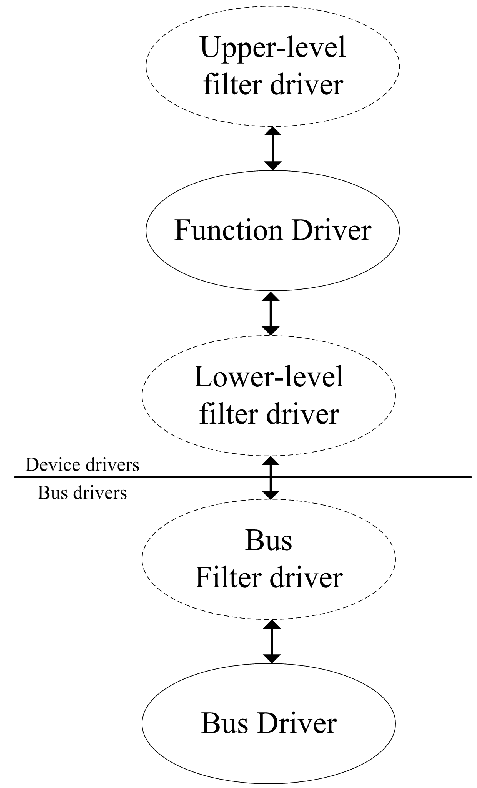
\includegraphics[width=0.4\linewidth]{./graph/io-stack-filter}
\caption{驱动程序堆栈和过滤器驱动程序}
\label{fig:io-stack-filter}
\end{figure}

存在三种类型的过滤器驱动程序:

\begin{enumerate}
\item
总线过滤器驱动:过滤、处理总线事件,将总线的硬件信号转换为驱动程序能够处理的总线事件,管理总线上挂载的设备对象,为总线设备加入新的功能。
\item
底层过滤器驱动:位于功能型驱动程序之下,用于改变设备展现给功能型驱动程序的硬件行为,使功能型驱动程序按照期望的方式运行。
\item
上层过滤器驱动:处于功能型驱动程序之上,过滤应用程序发送给设备的由IO管理器封装为IRP的IO请求。过滤到的IRP多为抽象程度高、硬件相关度低的IO请求。
\end{enumerate}

本论文实现的机械硬盘存储卷的过滤器驱动,是一种存在于机械硬盘所属的驱动程序堆栈中的上层过滤器驱动程序。

\section{缓存页面替换算法}
\label{sec:cache_algorithm}

伴随着应程序访问存储设备,不断会有新的数据加入到缓存空间。当缓存中已经没有空闲的存储空间,而此时又有新的主存数据可以加入时,就需要使用缓存页面替换算法选择性地释放空间,从而容纳新进数据。

常用的缓存页面替换算法按照替换策略可分为基于时间和基于频度的两类,本缓存系统对这两种类型的替换算法都进行了实现。除此之外,本论文还改进了LRU缓存页面替换算法,改进后的算法综合考虑了缓存块访问时间和访问频度因素。缓存系统运行时,可任意从这三种中选择其中一种使用。

\subsection{基于访问时间的LRU(Least Recently Used)系列替换算法}

LRU替换算法\cite{LRU}通过缓存块最后一次访问距离当前的时长进行决策。当缓存没有空闲空间时,替换出最近最不使用的(距上次访问时间最长的)缓存块。

虽然LRU替换算法根据访问时间进行替换决策,但实现时并不需要为每个缓存块记录访问时间,而是使用链表的方式组织缓存块:根据缓存块在链表中的位置记录缓存块最后一次访问距离当前的时长。

缓存块链表存在冷、热两端。当存在空闲的缓存块时,新缓存块会由热端加入。运行中被访问的缓存块从链表中的任意位置移动到热端。当需要加入新缓存块而缓存链表又已经满时,从链表的冷端移除缓存块,替换数据后加入到链表热端(图\ref{fig:replace-algo-lru})。从热端到冷端,链表中的元素均按照最近一次访问时间的递减顺序排列。

\begin{figure}[!htb]
\centering
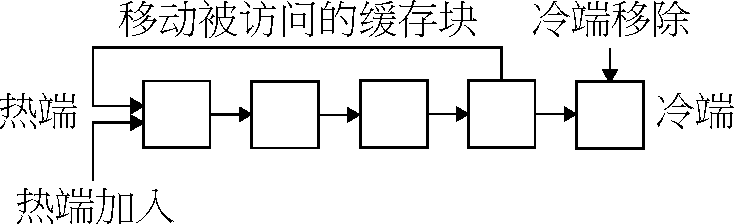
\includegraphics[width=0.6\linewidth]{./graph/replace-algo-lru}
\caption{使用链表的LRU缓存替换算法}
\label{fig:replace-algo-lru}
\end{figure}

LRU替换算法实现简单,能够以很低的性能开销适应变化的数据访问。存在的缺点是,对于考虑数据的长期访问特性没有做出很好的处理。最近使用的缓存块可能并不会被经常访问;经常访问的数据也可能因为暂时不使用而被换出,导致更需要留在缓存中的数据块被替换出去。

\subsection{基于使用频度的LFU(Least Frequently Used)系列替换算法}

LFU替换算法\cite{LFU}利用缓存块的访问频数进行决策。当缓存中不存在空闲的缓存块时,替换出历史访问频度最小的缓存块。

新加入的缓存块初始访问频度为1,随系统运行动态调整访问频度。为了在最短时间找到被替换出的缓存块,实现中使用小顶堆数据结构进行缓存块的组织,堆顶元素总是访问频度最低的元素,随时可以被替换出去。

LFU算法需要为每个缓存块设置一个记录访问频度的区域,以保存访问次数。使用了小顶堆数据结构实现替换策略,实现难度略高于LRU。缺点是需要一定策略对计数器进行清零,否则计数器只增不减会导致某些曾经被频繁访问的缓存块无法及时地被清理出去;新加入缓存块访问频度低,在缓存中停留较短时间后就会被替换出去。

\subsection{综合考虑时间和访问频度的替换算法}

上述两种缓存页面替换算法在选择缓存块时,都存在只考虑最后一次的访问时间或使用频度等某一项因素进行评估的缺陷。为了克服这种缺陷,本论文使用了一种综合考虑访问时间和使用频度的替换算法,该算法实现简单,且测试结果表明命中率优于LRU和LFU替换算法。以下是该算法的缓存块组织方式和处理逻辑:

替换算法使用冷、热两个链表管理缓存块(图\ref{fig:replace-algo-1}),初始状态下两个链表均为空,代表缓存中还没有开始缓存数据。类似于LRU,每个链表都存在冷、热两端,缓存块在链表中的位置代表了缓存块最近一次访问的时间。两个链表的容量上限之和代表了缓存的总容量。
\begin{figure}[!htb]
\centering
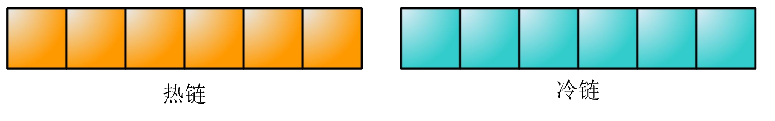
\includegraphics[width=0.6\linewidth]{./graph/replace-algo-1}
\caption{替换算法使用两个链表管理缓存块}
\label{fig:replace-algo-1}
\end{figure}

当冷链表不为满时,新到来的缓存块首先会被加入到冷链表的热端,在运行过程中会统计每个缓存块的访问计数(初始为1)。如果某个缓存块被访问,该缓存块无论在冷链还是热链都会被移动到该链表的热端,并且访问计数增加1。图\ref{fig:replace-algo-2}展示了缓存块以A->B->C->D->E的字母表顺序加入缓存后的组织状态。
\begin{figure}[!htb]
\centering

\includegraphics[width=0.6\linewidth]{./graph/replace-algo-2}
\caption{新到来的缓存块加入到冷链表}
\label{fig:replace-algo-2}
\end{figure}

随着缓存系统的运行以及缓存块的不断加入。当冷链表已满,而又要加入新的缓存块时。则需从冷链中移出一部分缓存块以释放空间,新的缓存块仍旧会被加入到冷链的热端。缓存算法会判断被移出缓存块的引用计数,如果其引用计数大于等于2,则清零其引用计数,并加入到热链表的热端;否则该缓存块空间将会被释放。图\ref{fig:replace-algo-3}展示了加入块G移出块A的过程。
\begin{figure}[!htb]
\centering

\includegraphics[width=0.6\linewidth]{./graph/replace-algo-3}
\caption{冷链表满时加入缓存块的处理策略}
\label{fig:replace-algo-3}
\end{figure}

新缓存块的持续到来导致冷链表中的缓存块不断被移动到热链表,热链表也会逐渐变满。当热链表中也不存在空闲空间时,加入新缓存块,热链表冷端的缓存块会像图\ref{fig:replace-algo-3}中冷链表的冷端的缓存块一样被换出。从热链中被换出的缓存块的引用计数会被清零,然后加入到冷链表的热端,重复图\ref{fig:replace-algo-3}的过程。整个过程在图\ref{fig:replace-algo-4}中描述。
\begin{figure}[!htb]
\centering
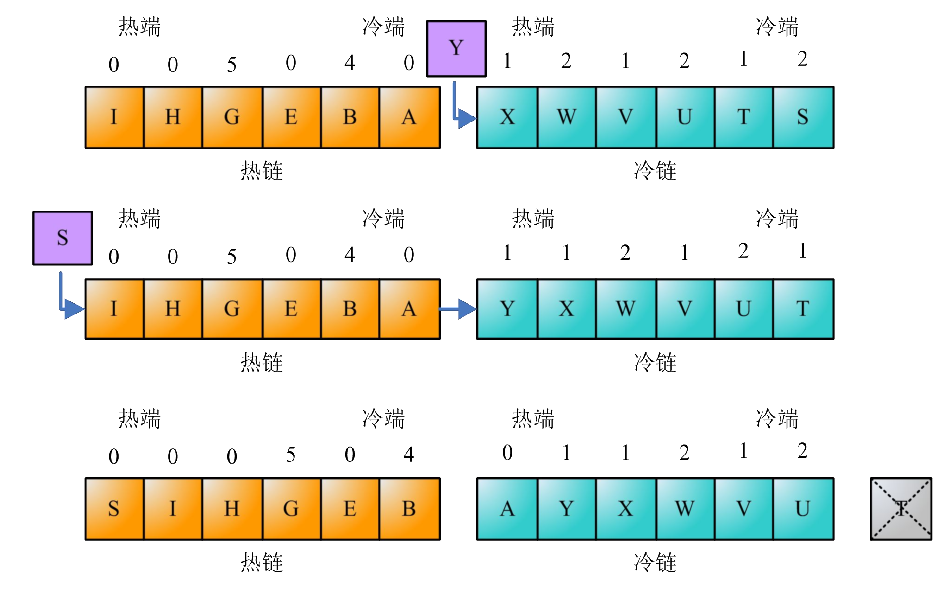
\includegraphics[width=0.7\linewidth]{./graph/replace-algo-4}
\caption{冷热链表均满时加入缓存块的处理策略}
\label{fig:replace-algo-4}
\end{figure}

本替换算法的核心思想是:冷、热链表内部完成LRU替换算法;冷、热链表之间完成LFU替换算法。单独观察冷或热链表,实质就是一个LRU算法管理的链表。缓存块在两个链表之间移动时,考虑到了访问频度的因素,这一点则反映了LFU替换算法的思想。

\section{缓存映射策略}
\label{sec:cache_mapping}

缓存映射策略指的是从主存空间到缓存空间之间的映射关系,缓存映射策略的选择直接决定了缓存系统的实现结构和运行效率。目前,存在三种使用场景最多的缓存块映射策略\cite{cachemap2013}。

\subsubsection{直接相联映射}

主存储器中的每一块空间,都被映射到了缓存中的某块指定的存储空间中。每个缓存块关联了主存中的一个或多个存储空间(图\ref{fig:cache-map-1})。

\begin{figure}[!htb]
\centering
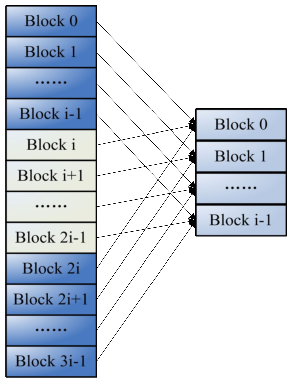
\includegraphics[width=0.4\linewidth]{./graph/cache-map-1}
\caption{直接相联映射}
\label{fig:cache-map-1}
\end{figure}

映射规则:
\begin{itemize}
\item 按相同大小的数据块划分主存与缓存空间。
\item 主存容量和缓存容量是整数倍的关系。将主存空间按缓存容量进行分区,主存每个区域内的块数等同于总的缓存块数。 
\item 主存中某区的一块数据,只能存入缓存中偏移与该块数据距离主存区域开始的距离相同的位置。
\end{itemize}

以主存地址x映射到缓存地址y为例,则x和y满足如下关系。
y = x mod m	(M为缓存的总大小)
直接映射方式的优点是实现简单,可以使用主存地址直接计算出对应的缓存地址,不存在查找过程。缺点是缓存中的每个存储块通常对应主存中多个固定的存储块,运行中如果存在多个块同时被访问会产生缓存替换策略被频繁调用的情况。因此,直接映射适合缓存容量为主存的30\%以上时采用,一般应用于超大型系统。

\subsubsection{全相联映射}

与直接相联的固定映射方式相反,全相联映射缓存中的每一块都可映射给将主存的任一块数据(图\ref{fig:cache-map-2})。

\begin{figure}[!htb]
\centering
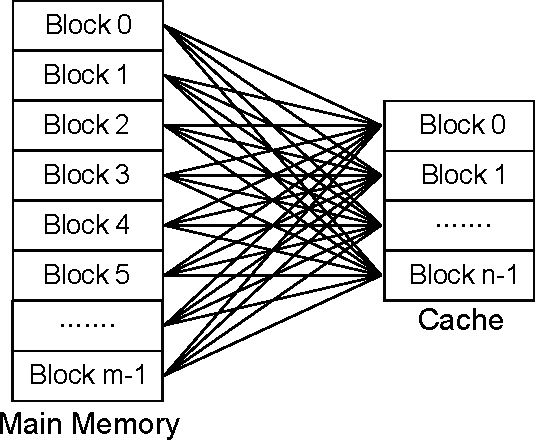
\includegraphics[width=0.4\linewidth]{./graph/cache-map-2}
\caption{全相联映射}
\label{fig:cache-map-2}
\end{figure}

映射规则:
\begin{itemize}
\item 按相同大小的数据块划分主存与缓存空间。
\item 缓存的每一块都可映射给主存的任意一块数据。缓存块总数是N,主存块总数是M时,存在多达N×M种的映射关系。
\end{itemize}

全相联映射的优点是主存和缓存的容量没有限制,只需按照相同大小的数据块进行组织,缓存空间利用灵活。缺点是在不使用额外的索引数据结构的情况下,当查询主存中的某个数据块是否被缓存时,需要遍历所有缓存块进行查找。为提高查找效率,必须要使用辅助的查找数据结构建立索引,使用额外的空间存储索引也必不可少。

\subsubsection{组相联映射}

主储存器的每一组都与缓存中的某一组相对应,组内的每个块与缓存组内的任意一个存储块相映射(图\ref{fig:cache-map-3})。

映射规则:
\begin{itemize}
\item 按相同大小的数据块划分主存与缓存空间。
\item 主存与缓存以相同数量的数据块划分成组。
\item 主存内组的数目是缓存内总组数目的整数倍。
\end{itemize}

\begin{figure}[!htb]
\centering
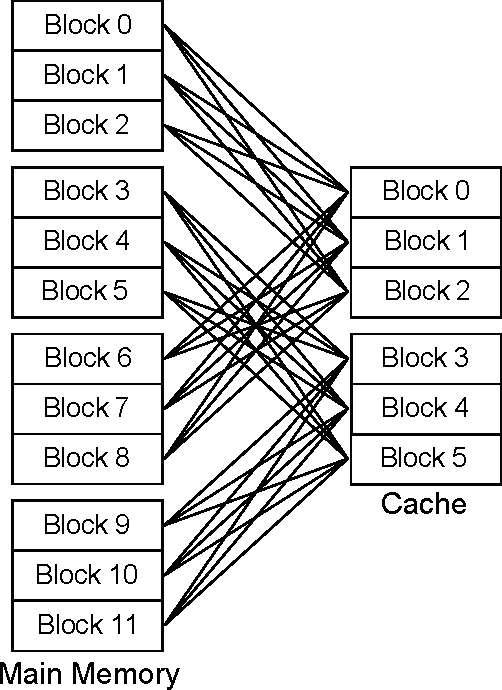
\includegraphics[width=0.4\linewidth]{./graph/cache-map-3}
\caption{组相联映射}
\label{fig:cache-map-3}
\end{figure}

当检测缓存是否命中时,先使用主存地址求出其唯一对应的缓存组,既主存组内的某一块只能存入同一组号的缓存组内。相关联的两组内各存储块之间的映射关系任意,这一方面类似于全相联映射。组与组之间的映射关系固定,这一方面类似直接相联映射。

一般会从三个角度比较这几种映射策略。
\subsubsection{索引速度}
直接映射可以直接计算出缓存地址,不需要查找,速度最快;组相联方式则需要查找对应的缓存组,速度次之;全相联映射的查询最为复杂。
\subsubsection{缓存利用率}
全相联方式主存和缓存块之间的映射关系任意,缓存利用率最高;组相联方式组内映射任意,但是组间相互独立,利用率次之;直接映射缓存中的每个缓存块与主存中的一个或多个存储块相关联,利用率最低。
\subsubsection{实现难度}
直接映射方式计算复杂度最低,适合硬件实现;组相联方式和全相联映射方式的实现难度取决于使用的索引数据结构。组相联方式可以在组内块数量较少时使用遍历的方法,这种实现也相对简单。

\section{缓存索引数据结构}
\label{sec:cache_indexing}

缓存系统使用缓存索引数据结构查询某个主存块是否被缓存、定位缓存块在缓存中的位置。缓存系统所选用的映射策略,决定了对应的缓存索引数据结构。

使用直接相联映射结构,主存储器中的每个数据块,根据地址的映射关系,对应了缓存中唯一的一个缓存块。因此,使用直接相联映射策略时,不需要额外的缓存索引结构支持缓存块的查找,使用主存地址直接计算就可以得知该主存块是否被缓存。

使用全相联映射结构,主存储器中的每个数据块和缓存中的每个数据块的存储地址之间没有任何的关系,主存储器的一个数据块可以映射到缓存中的任意某个缓存块的位置。使用全相联映射结构,进行缓存块的查找时,为了避免遍历查找带来的延迟,就不得不需要某种额外的索引数据结构定位主存储块映射的缓存块地址。

如果选用组相联方式,则是折中了直接相联和全相联两种映射结构。组相联映射将主存储器和缓存空间分成个数相同的存储块组,思想类似于直接映射。主存和缓存相联的两组内的主存块和缓存块之间的任意映射关系又等同于全相联映射的思想。在设计缓存系统的过程中需要决定分组的大小:当每个分组内的缓存块数量较少时,查找时可使用实现简单的遍历方法,不需要额外的索引数据结构;当分组内缓存块数量较多时,则和全相联映射一样,需要额外的索引数据结构避免查找带来的长的延迟。

从组织方式上分,索引数据结构分为单级结构、多级结构和树形结构三种类型。

\subsection{单级有序索引}
单级有序索引,顾名思义,就是只需要查询一级,便可以完成从主存储器地址到缓存地址空间的转换,索引结构是线性的。通常使用数组或是链表这类简单数据结构即可满足需求。

\subsubsection{数组方式}
使用静态数组为缓存中的每一个缓存块建立一个索引标签,标签记录了缓存块映射所到的主存储块,未映射时标记为空。索引需要遍历数组元素进行查找。优点是实现简单。缺点是需要在初始化阶段给所有的缓存块建立索引标签,如果缓存空间大,则需要的空间太多,索引速度慢。

\subsubsection{链表方式}
使用双向链表为每一个已经使用的缓存块建立一个索引标签,链表中的所有标签按照缓存地址的大小顺序排列。通过加入、删除和更新链表元素的方式实现缓存映射的更新。相对数组,链表可以在运行时动态分配所需空间。但索引时仍需要遍历所有元素。

\subsection{多级有序索引}

多级索引,是对单级索引空间从横向或者纵向进行多级划分,解决超大容量缓存空间的检索效率问题。由于几个不同种类的单级索引组合在一起,就可以构成一种新的多级索引方法。因此,多级索引的种类繁多。

\subsection{B+树索引}
B+树\cite{bplustree2012}是一种树形索引数据结构,通常用于数据库系统设计和文件系统在磁盘上索引的实现中。B+树的插入与删除操作的 时间复杂度非常稳定。而且因其自底向上的元素插入方式,与红黑树恰恰相反。

\subsubsection{B+树的节点结构}

B+树中的节点内部都会保存一组有序的索引和一组有序的节点指针。如果B+树的阶(order)是m,那么除了当只有一个叶子节点时,每个节点都最少包含m/2个,最多包含m-1个索引。内部节点的节点指针的数目总是比索引的数目多一个,内部节点的节点指针总是指向下一层的内部节点。所有叶子节点处于同一层的高度,其内部的索引数目和有效元素指针(节点指针)的数目相同,节点指针指向被索引的数据。图\ref{fig:bplus-tree}展示了一棵阶为4的B+树。

通常称B+树内部节点保存的每个索引值为分离值。例如,某个内部节点存在两分离值(元素)$a_1$和$a_2$,则其必须存在三个子指针指向其子树:左子树的所有节点的元素值均小于$a_1$,中间子树所有节点的元素值处于$[a_1,a_2)$区间,右子树的所有节点的元素值均大于等于$a_2$。

\subsubsection{B+树的查找算法}

B+树的查找算法类似于排序二叉树:从根节点开始,自顶向下遍历树的节点,根据要查找数据的索引值决定选择分离值哪一边的节点指针。使用子指针进入下一层内部节点,直到进入某个叶子节点。遍历叶子节点的所有元素,查找索引值,如果存在相同元素则找到,否则B+树中不存在查询索引。

\subsubsection{B+树的插入算法}

当节点内元素的数目不属于B+树节点结构的可接受的范围时,这个B+树节点处于违规状态。节点内节点指针的最小数量必须大于m/2。B+树的插入过程要处理节点因包含过多元素而违规的情况,插入过程为:
\begin{enumerate}
\item 根据数据索引值,查找适合的元素插入叶子节点。
\item 将元素插入到叶子节点内部的合适位置上。
\item 此时的叶子节点如果未因包含过多元素而违规,处理结束。
\item 如果此时的叶子节点包含的元素过多,则分裂为两个叶子节点,这两个节点必将拥有最小数目元素。分裂操作会导致上一内部层节点元素指针数目增加,因此需要递归向上处理到根节点。如果根节点也因包含过多元素而被分裂,则创建新的根节点,树的高度也因此而增加。
\end{enumerate}

\subsubsection{B+树的删除算法}

B+树的删除过程要处理节点违规的情况,删除过程为:

\begin{enumerate}
\item 根据索引值,查找到包含被删除元素的叶子。
\item 删除叶子节点内的待删除元素。
\item 如果此时叶子节点没有因元素过少而违规,处理结束。
\item 此时节点可能处于以下两种违规的状态之一,递归向上处理违规的叶子节点,直到不存在违规节点:
\begin{enumerate}
\item 节点的左、右兄弟节点,在不变为违规节点的前提下,可以把一或多个子节点移动到处于违规状态的节点,使其变为合法的节点。在移动子节点内元素后,必然要更新相应节点的分离值,并向上递归处理。
\item 节点的左、右兄弟节点内的元素个数均处于合法个数的下界。这种情况下,将当前节点和左或右兄弟节点合并,再平均分裂为两个节点。更新相应节点的分离值,持续这一过程直到当前节点合法或者合并到达根节点。
\end{enumerate}
\end{enumerate}

\begin{figure}[!htb]
\centering

\includegraphics[width=1\linewidth]{./graph/bplus-tree}
\caption{B+树结构}
\label{fig:bplus-tree}
\end{figure}

\section{回写策略}
\label{sec:wb_strategy}

对于应用程序的读请求,主存中的数据不会被改变,因此不存在数据一致性的问题。然而对于应用程序的写请求,需要决定是直接将写请求应用到主存储上还是延迟后再进行写更新,这种决定何时写回的策略被称之为回写策略\cite{writeback2014}。

本节将会介绍工程实现中使用最为广泛的三种回写策略:写穿法、写回法和写一次法的原理和实现方式。本论文实现的缓存系统实现了写穿法、写回法两种回写策略,运行时只能选取其中一种策略运行。

\subsection{写穿法(Write Through)}
\begin{figure}[!htb]
\centering
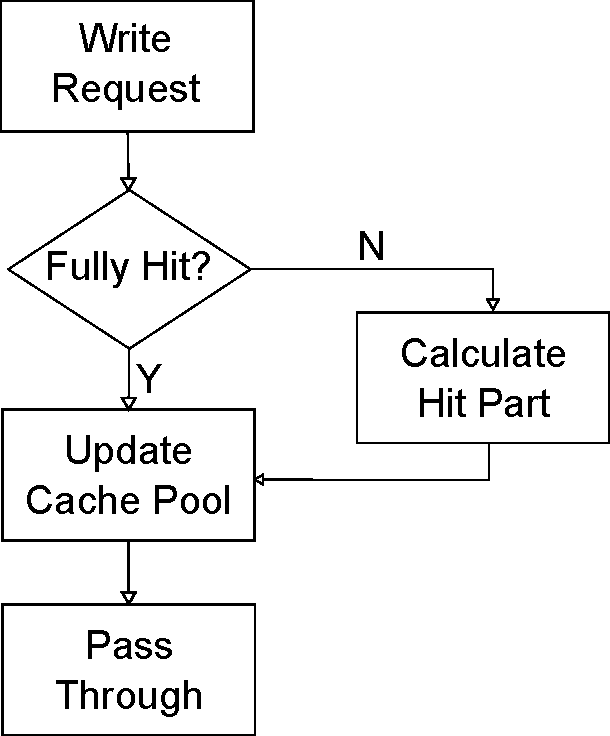
\includegraphics[width=0.4\linewidth]{./graph/write-through}
\caption{写穿法处理策略}
\label{fig:write-through}
\end{figure}

写穿法\cite{writethrough2010}对于接收到的写请求,同时应用于机械硬盘和固态硬盘缓存。由于机械硬盘和固态硬盘缓存数据是同时写入的,因此无需考虑断电造成的数据丢失问题,也无需为每个缓存块设置标志位记录此缓存块是否被修改过(图\ref{fig:write-through})。

写穿法这种回写策略的缺点是,运行这种回写策略的缓存系统不但无法提升应用程序的写操作的IO性能,相反的,还会造成写性能一定程度的降低。这是因为,如果没有缓存系统,应用程序的写操作直接应用到机械硬盘上即可;存在缓存系统,除了应用到机械硬盘,还要使用写请求的数据更新固态硬盘缓存中命中部分的数据,总的处理时间相对没有缓存反而更长。

\subsection{写回法(Write Back)}
\begin{figure}[!htb]
\centering

\includegraphics[width=0.4\linewidth]{./graph/write-back}
\caption{写回法处理策略}
\label{fig:write-back}
\end{figure}

写回法\cite{writeback2008}对于接收到的写请求,只将写操作应用于固态硬盘缓存,更新后立即完成写操作请求。写回法需要为每个缓存块设置一个修改位标志,更新后将修改位标志置位,并将缓存块指针加入到回写队列(图\ref{fig:write-back-queue}),回写线程在延迟一定时间后同步机械硬盘数据,同步后清除修改位标志。缓存页面替换算法运行时,不能选择替换修改位标志被置位的数据块。

\begin{figure}[H]
\centering
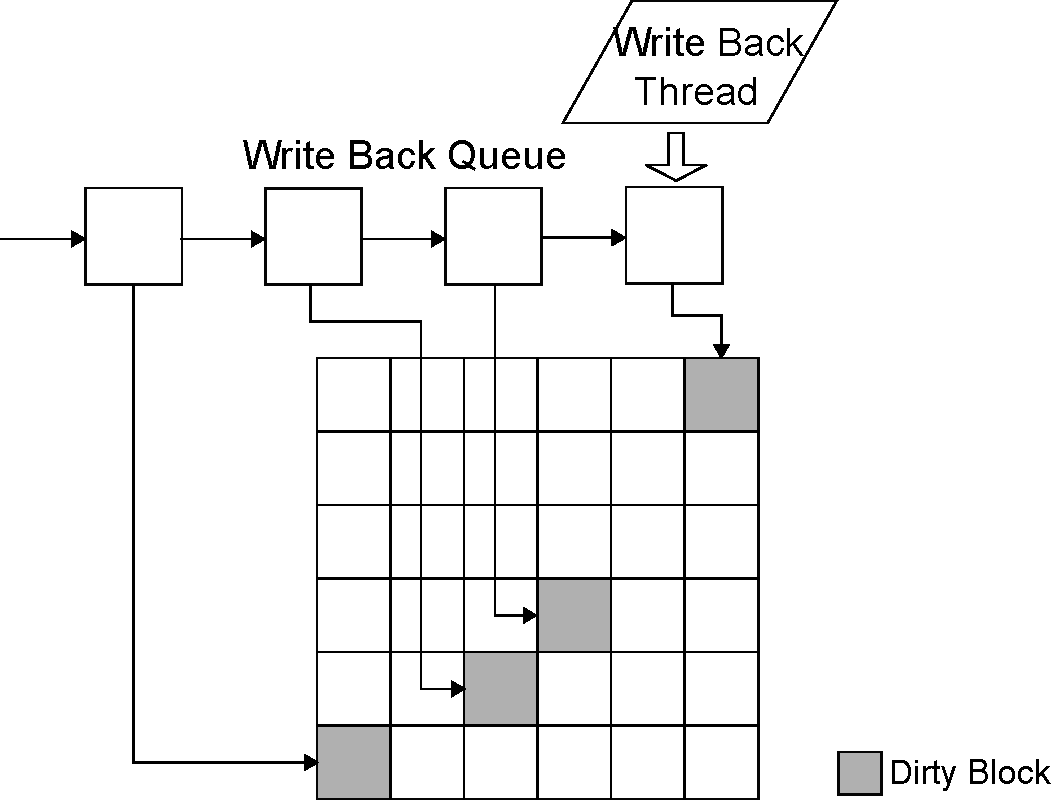
\includegraphics[width=0.6\linewidth]{./graph/write-back-queue}
\caption{指向脏数据块的回写队列}
\label{fig:write-back-queue}
\end{figure}

回写队列的大小是固定的。随着脏数据块的加入,当回写队列满时,会触发回写线程进行写回操作。回写线程将队列中的所有脏缓存块刷回机械硬盘。同样的,当线程接收到‘写回所有’或‘终止线程’信号时,也会进行刷写所有脏缓存块回机械硬盘的操作(图\ref{fig:write-back-thread})。

\begin{figure}[H]
\centering
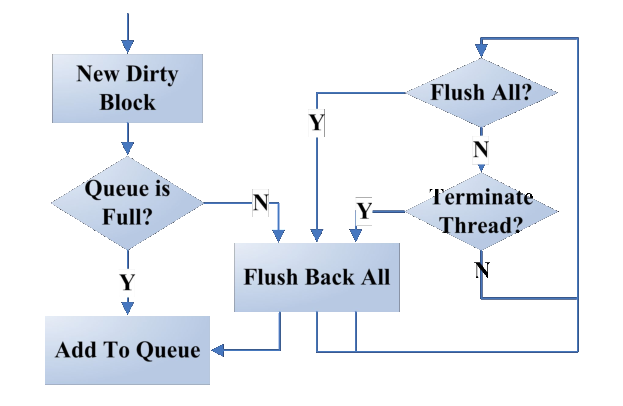
\includegraphics[width=0.6\linewidth]{./graph/write-back-thread}
\caption{回写线程的回写逻辑}
\label{fig:write-back-thread}
\end{figure}

\subsection{写一次法(Write Once)}
写一次法是一种融合了写穿和写回两种方法的回写策略。它的特点是,如果对某个缓存块的写请求命中,只在第一次写更新缓存块时使用写穿策略更新机械硬盘的数据,之后的每次写操作都和写回法一样,只修改缓存内的数据,机械硬盘数据会被延迟写回更新。

实现写一次法,需要为每个缓存块记录该缓存块曾被改写过的次数。

%% ----------------------------------------------------------------------
%%% END OF FILE
%% ----------------------------------------------------------------------

%% ----------------------------------------------------------------------
%% START OF FILE
%% ----------------------------------------------------------------------

\chapter{设计实现}
\label{cha:mainmatter}

本章介绍了论文提出的基于固态硬盘的缓存系统实现细节。从系统的整体架构框架出发,介绍抽象出的缓存算法的公共接口。接下来,给出了存储卷过滤器驱动程序的实现细节,以及缓存系统是如何实现支持使用超长缓存块组织缓存空间。最后,描述了应用层用户配置工具所提供的控制命令和对应的IOCTL代码。

\section{系统整体架构}
\label{sec:system_overview}

缓存系统的实现可分为存储卷过滤器驱动程序、缓存系统和用户配置工具几部分(图\ref{fig:sys-overview})。

\begin{figure}[H]
\centering
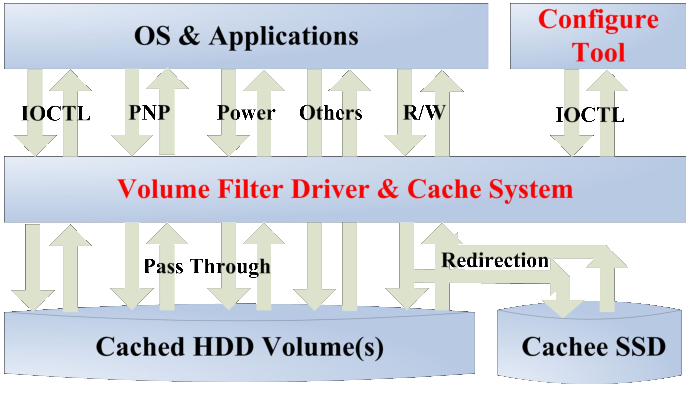
\includegraphics[width=0.6\linewidth]{./graph/sys-overview}
\caption{缓存系统结构图}
\label{fig:sys-overview}
\end{figure}

\begin{itemize}
\item
存储卷过滤器驱动程序:过滤用户程序和操作系统对HDD卷的读写请求,供缓存算法进行SSD缓存时使用。
\item
缓存逻辑实现模块:完整的缓存系统实现,包括读写请求处理线程、缓存页替换算法、回写线程队列、缓存块索引数据结构等部分。这一模块的技术细节属于系统实现的关键技术,在上一章已经介绍。
\item
用户配置工具:提供给用户一定的缓存系统控制接口,通过IOCTL命令与驱动程序进行交互,控制过滤器驱动程序和缓存算法的运行状态。
\end{itemize}

存储卷过滤器驱动程序和缓存逻辑实现模块是系统的核心部分。这两部分虽然在逻辑上分离,但是互相依赖且存在非常多的数据交互。因此为了降低实现难度、减少模块间交互带来的性能损失,这两部分实现于同一个Windows内核模块之中(图\ref{fig:sys-flt-arch})。

\begin{figure}[H]
\centering
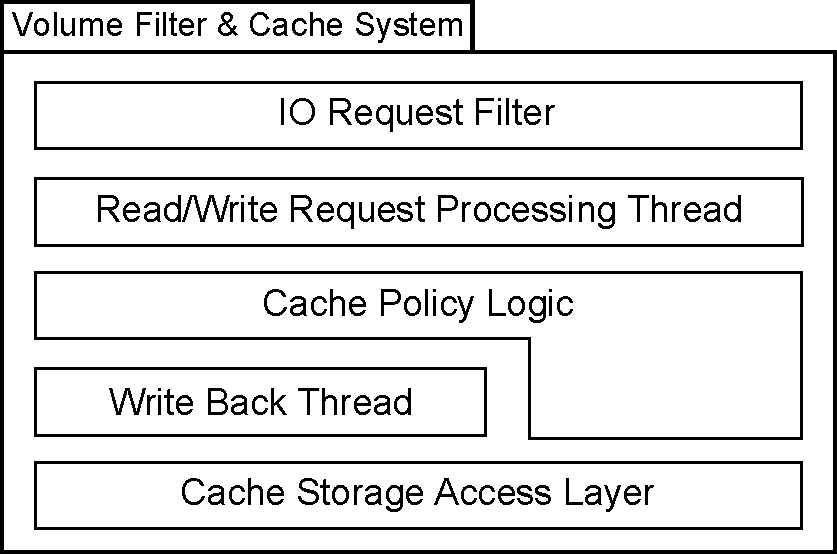
\includegraphics[width=0.6\linewidth]{./graph/sys-flt-arch}
\caption{存储卷过滤器驱动程序架构}
\label{fig:sys-flt-arch}
\end{figure}

\begin{itemize}
\item
IO请求(IRP)过滤器:过滤存储卷设备所在IO栈上的所有类型IRP,将读写类型的IRP加入读写队列;其他类型的IRP只关注存储卷上线、移除等几种特定的类型。
\item
读写请求处理线程:通过与缓存系统交互,处理加入读写队列的IO请求。
\item
缓存算法逻辑:使用SSD缓存池中的数据处理针对HDD的读写请求;利用从HDD得到的数据,结合缓存页面替换算法,更新SSD缓存池。
\item
回写线程:实现了写回(Write Back)和写穿(Write Through)两种回写策略,定期将缓存池中未同步的脏数据写回到HDD。
\item
缓存介质访问层:管理作为缓存的SSD存储卷的空间分配和读写相关操作。
\end{itemize}

%% ----------------------------------------------------------------------

\section{缓存算法通用接口}
\label{sec:cache_interface}

缓存系统实现中包含了LRU、LFU和论文提出的缓存页面替换算法。无论哪种页面替换算法所要达到的目的,以及提供给过滤器驱动程序的接口都一致。为了减少系统实现中的冗余代码,论文实现过程中将缓存算法的通用接口进行了抽象,每种替换算法只要按照通用接口进行实现,系统代码就可以通过C语言宏开关的方式方便切换缓存替换算法。

通用接口分为内部和外部两类接口函数。外部接口将会被暴露给过滤器驱动程序,完成缓存系统的功能;外部函数接口的实现代码中会调用内部函数接口,虽然不同替换算法的替换策略不同,但实现中页面替换的逻辑流程仍然是相同的,因此可以为不同的算法抽象出相同的内部函数接口,减少冗余代码、方便缓存系统进行缓存替换算法间的切换。

\subsection{数据结构}

缓存系统用到了两种结构体:缓存块结构体用于映射主存块和缓存块,缓存池结构体用于组织管理缓存存储空间。

\begin{itemize}

\item 缓存块(CACHE\_BLOCK)
\\映射SSD缓存块和HDD主存块,代表了最小的缓存存储单元。
\begin{lstlisting}
typedef struct _CACHE_BLOCK
{
    ULONGLONG Index;
    ULONGLONG StorageIndex;
    BOOLEAN   Modified;
}CACHE_BLOCK, *PCACHE_BLOCK;
\end{lstlisting}
Index是HDD主存块的索引,标记了缓存块所对应的主存块在HDD中的位置。StorageIndex是SSD缓存块的索引,记录了该缓存块在缓存空间中的位置。Modified是更改标志:当回写策略是写回(Write Back)时,标记当前缓存块是否与主存同步,TRUE表示不同步需要回写,FALSE表示同步;回写策略是写穿(Write Through)时,更改标志没有意义。

\item 缓存池(CACHE\_POOL)
\\SSD缓存空间的存储块池,用于组织缓存存储块,记录缓存池的使用情况和统计信息。
\begin{lstlisting}
typedef struct _CACHE_POOL
{
    ULONG        Size;
    ULONG        Used;
    STORAGE_POOL Storage;
    ULONG32      ReadCount;
    ULONG32      WriteCount;
    ULONG32      ReadHit;
    ULONG32      WriteHit;
}CACHE_POOL, *PCACHE_POOL;
\end{lstlisting}
Size记录了缓存池内所包含的存储块总数,即缓存池的总空间大小。Used记录了缓存池内已使用存储块数量。Storage代表组织所有缓存存储空间的存储池,负责管理底层存储介质访问。ReadCount记录被缓存设备接收的读请求总数。WriteCount记录被缓存设备接收的写请求总数。ReadHit记录缓存的读请求命中总数。WriteHit记录缓存的写请求命中总数。

\end{itemize}

\subsection{外部函数接口}

外部函数接口被暴露给过滤器驱动程序,实现缓存系统的功能。

\subsubsection{InitCachePool}
初始化缓存存储块池结构体,申请存储池空间。
\begin{lstlisting}
bool InitCachePool (
    PCACHE_POOL CachePool
);
\end{lstlisting}

传入缓存池结构体指针。初始化成功返回TRUE,否则返回FALSE。

具体步骤为:
\begin{enumerate}
\item 初始化缓存池结构体的内部变量。
\item 初始化存储访问层和缓存存储设备。
\item 初始化缓存块索引数据结构B+树。
\item 初始化缓存页面替换算法所用到的数据结构。
\end{enumerate}

任何一步出现错误都撤回之前成功的操作,返回FALSE。所有步骤都成功才返回TRUE。

\subsubsection{DestroyCachePool}
销毁缓存存储块池,释放存储空间。
\begin{lstlisting}
void DestroyCachePool (
    PCACHE_POOL CachePool
);
\end{lstlisting}

具体步骤为:

\begin{enumerate}
\item 销毁缓存页面替换算法所用到的数据结构。
\item 销毁缓存块索引数据结构B+树。
\item 销毁存储访问层和停止缓存存储设备。
\end{enumerate}

\subsubsection{QueryAndCopyFromCachePool}
查询缓存池中的数据是否命中偏移为Offset,长度为Length的主存储设备读请求。
\begin{lstlisting}
bool QueryAndCopyFromCachePool (
    PCACHE_POOL CachePool,
    PUCHAR Buffer,
    LONGLONG Offset,
    ULONG Length
);
\end{lstlisting}

传入缓存池结构体指针,数据位置和数据指针。如果完全命中,拷贝数据到Buffer,返回TRUE;如果不命中,返回FALSE。

具体步骤为:
\begin{enumerate}
\item 检测读请求的起始和末尾部分是否存在不对齐的情况。
\item 计算完成该读请求所需要的所有缓存块。
\item 逐一检查所需的缓存块是否在缓存池中命中。
\item 如果没有全部命中,函数结束,返回FALSE。
\item 逐一拷贝命中的缓存块数据到传入的Buffer中。
\item 函数结束,返回TRUE。
\end{enumerate}

\subsubsection{QueryAndWriteToCachePool}
查询缓存池中的数据是否命中偏移为Offset,长度为Length的主存储设备写请求。
\begin{lstlisting}
bool QueryAndWriteToCachePool (
    PCACHE_POOL CachePool,
    PUCHAR Buffer,
    LONGLONG Offset,
    ULONG Length
);
\end{lstlisting}

传入缓存池结构体指针,数据位置和数据指针。如果完全命中,使用Buffer中的数据更新缓存池中的数据,返回TRUE;如果不命中,返回FALSE。

具体步骤为:
\begin{enumerate}
\item 检测写请求的起始和末尾部分是否存在不对齐的情况。
\item 计算此次写操作所涉及到的所有缓存块。
\item 逐一检查所需的缓存块是否在缓存池中命中。
\item 如果没有全部命中,函数结束,返回FALSE。
\item 使用传入Buffer中的数据,逐一更新所有涉及到的缓存块的数据。
\item 函数结束,返回TRUE。
\end{enumerate}

\subsubsection{ReadUpdataCachePool}
使用缓存页面替换算法,使用从HDD读出的数据更新缓存池。
\begin{lstlisting}
void ReadUpdataCachePool (
    PCACHE_POOL CachePool,
    PUCHAR Buffer,
    LONGLONG Offset,
    ULONG Length
);
\end{lstlisting}

传入缓存池结构体指针,数据位置和数据指针。Buffer中是从HDD读出的偏移为Offset,长度为Length的数据。如果缓存池还有空间,加入新缓存块到缓存池;否则使用缓存页面替换算法找出缓存块进行替换。

具体步骤为:
\begin{enumerate}
\item 检测HDD数据的起始和末尾部分是否存在不对齐的情况。
\item 逐一处理HDD数据所涉及的缓存块。具体步骤见图\ref{fig:read-update-pool},其中的虚线部分只有在写回模式时才会执行。
\end{enumerate}

\begin{figure}[H]
\centering
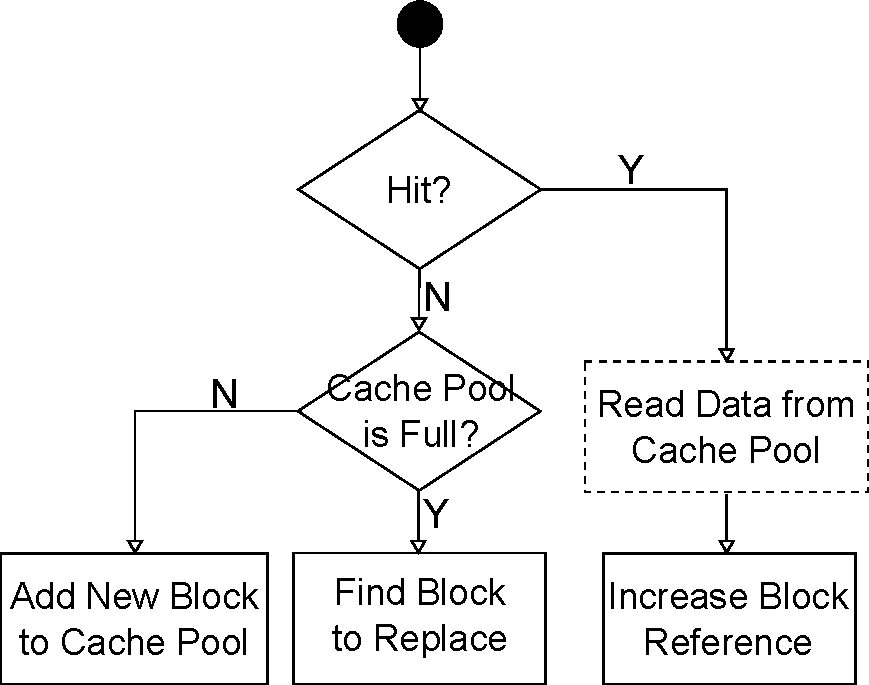
\includegraphics[width=0.6\linewidth]{./graph/read-update-pool}
\caption{读数据更新缓存池逻辑}
\label{fig:read-update-pool}
\end{figure}

\subsubsection{WriteUpdataCachePool}
使用缓存页面替换算法,利用已经写入HDD的数据更新缓存池。
\begin{lstlisting}
void WriteUpdataCachePool (
    PCACHE_POOL CachePool,
    PUCHAR Buffer,
    LONGLONG Offset,
    ULONG Length
);
\end{lstlisting}

传入缓存池结构体指针,数据位置和数据指针。Buffer中的数据是偏移为Offset,长度为Length的最新HDD数据。为保证数据的一致性,需要更新缓存中与HDD上最新数据(偏移为Offset,长度为Length)有重叠部分的数据。

具体步骤为:
\begin{enumerate}
\item 检测HDD数据的起始和末尾部分是否存在不对齐的情况。
\item 逐一处理HDD数据所涉及的缓存块。具体步骤见图\ref{fig:write-update-pool},其中的虚线部分只有在写回模式时才会执行。
\end{enumerate}

\begin{figure}[H]
\centering
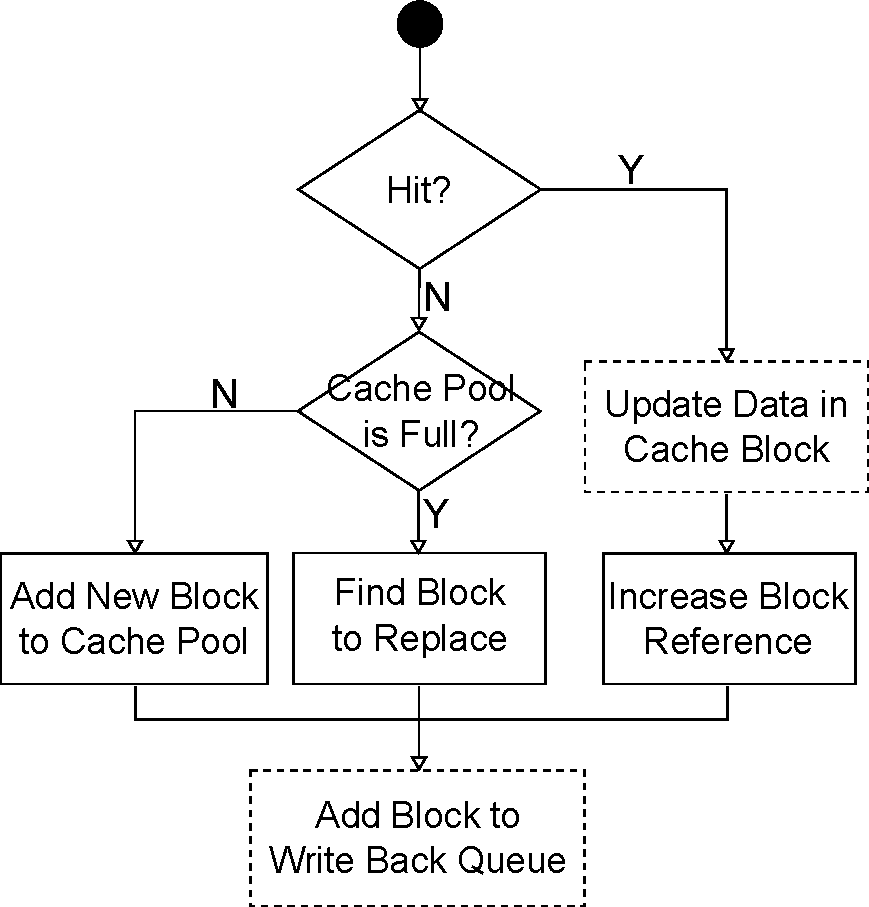
\includegraphics[width=0.6\linewidth]{./graph/write-update-pool}
\caption{写数据更新缓存池逻辑}
\label{fig:write-update-pool}
\end{figure}

\subsubsection{IsEmpty}
判断缓存存储块池是否为空。
\begin{lstlisting}
bool IsEmpty (
    PCACHE_POOL CachePool
);
\end{lstlisting}

传入缓存池结构体指针。如果为空返回TURE;否则返回FALSE。

\subsubsection{IsFull}
判断缓存存储块池是否存在空闲缓存块。
\begin{lstlisting}
bool IsFull (
    PCACHE_POOL CachePool
);
\end{lstlisting}

传入缓存池结构体指针。如果已满返回TURE;否则返回FALSE。

\subsection{内部函数接口}

内部函数接口在外部接口函数的实现代码中被调用。虽然不同缓存算法的替换策略不同,但总体逻辑流程相同,因此可为不同的算法抽象出相同的内部函数接口,方便在缓存替换算法之间切换。

\subsubsection{\_QueryPoolByIndex}
查询缓存存储块池中是否存在HDD数据索引为Index的缓存块。
\begin{lstlisting}
bool _QueryPoolByIndex (
    PCACHE_POOL CachePool,
    LONGLONG Index,
    PCACHE_BLOCK *ppBlock
);
\end{lstlisting}

传入缓存池结构体指针和HDD数据块索引。如果缓存命中,将该缓存块的指针赋值给ppBlock,返回TRUE;否则返回FALSE。不同的缓存页面替换算法使用了不同的缓存块组织结构,缓存池查询函数的实现也不相同,但是本质上都是在查询索引B+树上是否存在有相应的节点。

\subsubsection{\_\_GetFreeBlock}
从缓存存储块池中获取一个未使用的缓存块。
\begin{lstlisting}
PCACHE_BLOCK __GetFreeBlock (
    PCACHE_POOL CachePool
);
\end{lstlisting}

传入缓存池结构体指针。如果成功获取则返回指向空闲缓存块的指针,缓存池空闲缓存块计数减1;否则返回NULL。函数首先检查缓存池是否存在有空闲空间,如果存在,创建CACHE\_BLOCK结构体并从缓存存储设备上申请空间,返回结构体指针;否则返回NULL。

\subsubsection{\_AddNewBlockToPool}
加入新的缓存块到缓存池中。
\begin{lstlisting}
PCACHE_BLOCK _AddNewBlockToPool (
    PCACHE_POOL CachePool,
    LONGLONG Index,
    PVOID Data,
    BOOLEAN Modified
);
\end{lstlisting}

传入缓存池结构体指针,新缓存块数据及对应的HDD索引。当存储池存在空闲空间时,通过\_\_GetFreeBlock函数获取一个空闲的缓存块,索引赋值为Index,数据更新为Data所指向的数据,不同的缓存页面替换算法的实现会将缓存块加入到不同的缓存块组织结构中。Modified标记传入的数据是读类型还是写类型,使用写回策略时,包含写类型数据的缓存块需要加入到回写队列以便进行延迟回写。如果成功加入缓存池,返回新创建的缓存块指针;否则返回NULL。

\subsubsection{\_FindBlockToReplace}
从不存在空闲空间的缓存池中找出一个可替换的缓存块。
\begin{lstlisting}
PCACHE_BLOCK _FindBlockToReplace (
    PCACHE_POOL CachePool,
    LONGLONG Index,
    PVOID Data,
    BOOLEAN Modified
);
\end{lstlisting}

传入缓存池结构体指针,新缓存块数据及对应的HDD索引。该函数调用的前提是缓存块存储池已经不存在空闲空间。函数利用缓存页面替换算法从缓存池中选取出一个可替换的缓存块进行数据的替换。Modified标记传入的数据是读类型还是写类型,使用写回策略时,包含写类型数据的缓存块需要加入到回写队列以便进行延迟回写。如果替换成功,返回数据被替换的缓存块指针;否则返回NULL。

\subsubsection{\_IncreaseBlockReference}
增加缓存块的访问计数。
\begin{lstlisting}
VOID _IncreaseBlockReference (
    PCACHE_POOL CachePool,
    PCACHE_BLOCK pBlock
);
\end{lstlisting}

传入缓存池结构体指针和缓存块指针。当某个缓存块被访问时,告知告知缓存页面替换算法该缓存块的访问计数增加1,以进行页面替换算法内部数据结构的更新。

%% ----------------------------------------------------------------------

\section{IO操作捕获函数逻辑}
\label{sec:capture_io_logic}

驱动程序通过重载卷过滤器驱动程序的分发函数达到捕获应用程序IO操作的目的。

\subsection{默认分发函数}

默认分发函数用于实现我们不需要使用的分发函数接口。对于本驱动不关心的IRP,仍需传递给底层的驱动程序才能保证程序的正常运行。
一个驱动程序可以为每个分发函数接口实现一个独立的分发函数。同样的,也可以用一个分发函数实现多种分发函数接口。默认分发函数就是一种被用来实现多种分发函数接口的函数。该函数直接跳过IO栈上当前驱动设备对象所处的位置,将IRP发送给更底层的驱动设备对象(图\ref{fig:df-default})。

\begin{figure}[H]
\centering
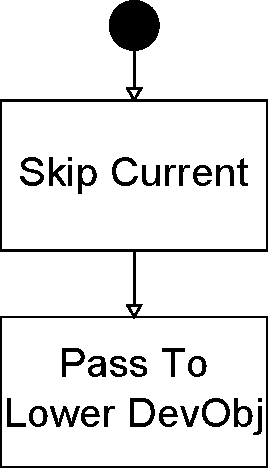
\includegraphics[width=0.20\linewidth]{./graph/df-default}
\caption{默认分发函数}
\label{fig:df-default}
\end{figure}

\subsection{电源事件分发函数}

电源事件分发函数实现了IRP\_MJ\_POWER分发函数接口。电源事件IRP包含了操作系统对硬件设备的电源操作,或是将硬件设备的电源的状态反馈给操作系统。
Windows操作系统允许传递SystemPowerState和DevicePowerState两种类型的电源状态信息。
本论文实现的存储卷过滤器驱动程序只关注SystemPowerState的PowerSystemShutdown电源事件。如图\ref{fig:df-power}所示,当包含系统即将关机信息的IRP被捕获后,电源事件分发函数会同步所有脏缓存块到HDD,并将IRP传递给更底层的设备对象;否则,跳过当前驱动设备对象,传递IRP给更底层的驱动设备对象。

\begin{figure}[H]
\centering
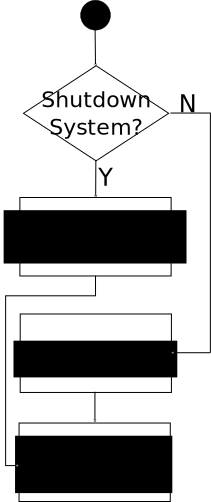
\includegraphics[width=0.25\linewidth]{./graph/df-power}
\caption{电源事件分发函数}
\label{fig:df-power}
\end{figure}

\subsection{IOCTL分发函数}

IOCTL分发函数实现了IRP\_MJ\_DEVICE\_CONTROL函数接口。IOCTL命令由Windows操作系统的IO管理器或是其他的内核驱动程序发送。大多数情况下,IOCTL类型的IRP是由用户层应用程序调用微软的Win32 API函数DeviceIoControl触发IO管理器产生的。
每当有存储卷初始化完毕将要上线时,IO管理器会给存储卷所在IO栈上的所有设备对象发送IRP\_MN\_QUERY\_REMOVE\_DEVICE的IOCTL命令。论文实现的存储卷过滤器驱动程序在过滤到此类型的IRP后,会向更底层的设备对象同步发送此IRP。确认存储卷已经上线后,检测上线的存储卷是否是目标卷。如果是目标卷,则查询目标卷的相关信息并进行相应的初始化操作,完成IRP请求;否则直接完成IRP请求(图\ref{fig:df-ioctl})。

\begin{figure}[H]
\centering
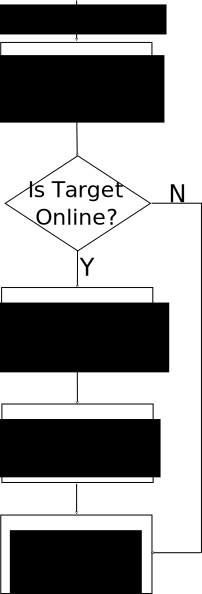
\includegraphics[width=0.25\linewidth]{./graph/df-ioctl}
\caption{IOCTL分发函数}
\label{fig:df-ioctl}
\end{figure}

\subsection{PnP事件分发函数}

PnP事件分发函数实现了IRP\_MJ\_PNP函数接口。PnP(Plug and Play)是总线在检测到硬件设备连接状态改变后,向总线驱动程序发送的一种总线信号。这种总线信号在被PnP事件管理器转换为相应类型的IRP后,会被发送给设备所在IO栈上的设备对象。
当存储卷即将被移除时,PnP事件管理器会给存储卷所在IO栈上的所有设备对象发送包含IRP\_MN\_REMOVE\_DEVICE信息的IRP。论文实现的存储卷过滤器驱动程序在过滤到此类型的IRP后,会向更底层的设备对象同步发送此IRP。确认存储卷被移除后,如果是被SSD缓存的卷,则停止工作线程、释放缓存索引占用的内存空间、从底层设备对象分离并移除当前驱动程序的设备对象,最终完成IRP请求(图\ref{fig:df-pnp})。

\begin{figure}[H]
\centering

\includegraphics[width=0.45\linewidth]{./graph/df-pnp}
\caption{PnP事件分发函数}
\label{fig:df-pnp}
\end{figure}

\subsection{读写分发函数}

存储卷的所有读和写操作都是通过IRP\_MJ\_READ和IRP\_MJ\_WRITE函数接口的实现函数完成的。论文实现的存储卷过滤器驱动程序使用一个读写分发函数统一实现了这两种函数接口。
该函数不会立即对包含读写请求的IRP进行处理(图\ref{fig:df-rw}),而是将IRP加入到驱动程序的读写请求队列中供驱动程序创建的读写线程处理,并返回IRP正在处理中的状态。

\begin{figure}[H]
\centering

\includegraphics[width=0.2\linewidth]{./graph/df-rw}
\caption{读写分发函数}
\label{fig:df-rw}
\end{figure}

读写线程检测到读写队列不为空时,从队列头部依次处理每个读写请求(图\ref{fig:df-rw-thread})。这样做的好处是可以使并行的读写操作串行化,避免了可能的数据访问冲突,同时还可以减少锁操作对性能的消耗。

\begin{figure}[H]
\centering

\includegraphics[width=0.75\linewidth]{./graph/df-rw-thread}
\caption{处理读写请求的内核线程}
\label{fig:df-rw-thread}
\end{figure}

读写线程中对读和写请求的处理逻辑相似但细节不同。图\ref{fig:df-proc-read}展现了读请求的处理逻辑。

\begin{figure}[H]
\centering

\includegraphics[width=0.8\linewidth]{./graph/df-proc-read}
\caption{读写线程的读请求处理逻辑}
\label{fig:df-proc-read}
\end{figure}

图\ref{fig:df-proc-write}展现了写请求的处理逻辑。写请求和读请求的处理都存在更新SSD缓存池的操作,但实现的细节并不相同:读请求直接使用读请求获得的HDD数据更新SSD;写请求依据回写策略的不同又可分为写穿(Write Through)和写回(Write Back)两类。写穿策略会先将写请求的数据先应用于HDD,再去更新SSD。写回策略直接使用写请求的数据更新SSD,回写线程负责将缓存中的脏数据同步回HDD。这两种回写策略在\ref{sec:wb_strategy}节被详细描述。

\begin{figure}[H]
\centering

\includegraphics[width=0.8\linewidth]{./graph/df-proc-write}
\caption{读写线程的写请求处理逻辑}
\label{fig:df-proc-write}
\end{figure}

%% ----------------------------------------------------------------------

\section{对超长缓存块的支持}

硬盘的最小存储单元是扇区,大小为512字节,因此Windows的IO管理器产生的读写请求会以512字节对齐。缓存系统中,缓存空间和主存储空间一般也会以512字节的大小进行划分。

但是,应用程序产生的磁盘读写请求操作的大小可能会达到几兆字节,对于这种请求,如果还以512字节进行划分,需要多次查询缓存池,对系统的性能影响很大。为了提升缓存系统性能,本论文实现的缓存系统支持超长缓存块:由IO管理器产生的,512字节对齐的读写请求无法改变;缓存空间使用512字节的倍数大小进行划分。这么做对于较大的读写请求,一方面可以减少分段的个数,降低多次查询缓存池对性能的影响;另一方面从缓存池内向外拷贝数据时,每次拷贝的数据量变大,拷贝效率更高。

如果读写请求的大小和缓存空间的划分不是以相同字节数目对齐,就需要在查询缓存池和拷贝缓存数据时解决读写数据不对齐的问题。如图\ref{fig:vsize-cache-block}所示,不对齐部分只可能出现在读写请求的开头(f\_broken)和结尾(e\_broken)部分。只需要特殊处理这两部分数据,其余部分按对齐方式正常处理即可。

\begin{figure}[H]
\centering
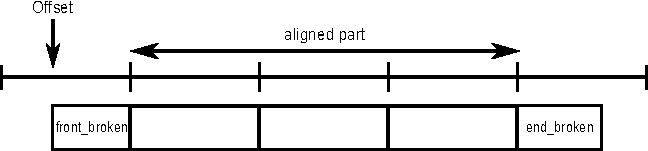
\includegraphics[width=0.8\linewidth]{./graph/vsize-cache-block}
\caption{请求长度与缓存块大小不对齐的情况}
\label{fig:vsize-cache-block}
\end{figure}

经实验验证,缓存块大小为4KB(8*512)时,性能提升效果最明显。

下面分别给出了读、写请求不对齐时缓存命中与不命中情况的处理方式:

\begin{itemize}

\item 读请求命中的处理
\begin{enumerate}
\item 检查对齐部分所属的数据块是否在缓存池中缓存。
\item 检查f\_broken和e\_broken部分的所属的数据块是否在缓存池中缓存。
\item 如果完全命中,在从缓存池中拷贝数据时,需要注意f\_broken和e\_broken部分拷贝数据时的偏移和长度。
\end{enumerate}

\item 读请求未命中的处理
\begin{enumerate}
\item 向下发送读请求,获得主存数据。
\item 只使用对齐部分所属的数据块更新缓存池。
\end{enumerate}

\item 写请求命中的处理
\begin{enumerate}
\item 检查对齐部分所属的数据块是否在缓存池中缓存。
\item 检查f\_broken和e\_broken部分的所属的数据块是否在缓存池中缓存。
\item 如果完全命中,在向缓存池中写入数据时,需要注意在写入f\_broken和e\_broken部分所属缓存块的偏移和长度。
\end{enumerate}

\item 写请求未命中的处理
\begin{enumerate}
\item 使用对齐部分所属的命中数据块更新缓存池。
\item 检查f\_broken和e\_broken部分所属的数据块是否命中。如果命中,写入并注意f\_broken和e\_broken部分写入数据时的偏移和长度;未命中,当回写策略是写回(Write Back)模式时,由于f\_broken和e\_broken部分的数据无法构成完整的缓存数据块,故而需要将这两部分数据直接写入主存储器。
\end{enumerate}

\end{itemize}

%% ----------------------------------------------------------------------

\section{用户配置工具}
\label{sec:config_utility}

系统提供了命令行的用户配置工具,在用户层和内核层的驱动程序进行交互。通过驱动设备对象提供的IOCTL命令,来完成两个方面的功能:
\begin{enumerate}
\item 配置缓存系统的运行状态。包括启动、停止和设置作为缓存的卷。
\item 获得缓存系统的统计数据。获得IO统计信息,如缓存使用、读写次数和命中率。
\end{enumerate}

配置工具启动后,依据用户输入的命令完成相应操作。工具提供有如下命令:

\begin{itemize}
\item start
\\描述:为某个指定的HDD存储卷开启SSD缓存。
\\使用:start  [disk\_number]  [volume\_number]
\\IOCTL:IOCTL\_DF\_START

\item stop
\\描述:停止某个HDD存储卷上的SSD缓存。
\\使用:stop  [disk\_number]  [volume\_number]
\\IOCTL:IOCTL\_DF\_STOP

\item stat
\\描述:获取某个存储卷的统计数据。包括读、写操作次数,缓存命中率以及使用情况。
\\使用:stat  [disk\_number]  [volume\_number]
\\IOCTL:IOCTL\_DF\_GET\_STAT

\item clear
\\描述:清除某个存储卷的统计数据。
\\使用:clear  [disk\_number]  [volume\_number]
\\IOCTL:IOCTL\_DF\_CLEAR\_STAT

\item quite
\\描述:设置驱动程序不向内核日志输出任何日志信息。
\\使用:quite
\\IOCTL:IOCTL\_DF\_QUIET

\item verbose
\\描述:开启驱动程序的向内核日志的所有日志信息输出。
\\使用:verbose
\\IOCTL:IOCTL\_DF\_VERBOSE

\item verify
\\描述:开启或关闭SSD缓存池内数据和HDD数据的一致性验证,默认是关闭的,开启对性能影响明显,只做调试使用。
\\使用:verify
\\IOCTL:IOCTL\_DF\_VERIFY

\item q
\\描述:退出用户配置工具。
\\使用:q
\end{itemize}

%% ----------------------------------------------------------------------
%%% END OF FILE
%% ----------------------------------------------------------------------

%% ----------------------------------------------------------------------
%% START OF FILE
%% ----------------------------------------------------------------------

\chapter{系统测试与结果分析}
\label{cha:exp_analysis}

\section{测试平台}
\label{sec:exp_platform}

操作系统 Microsoft Windows Server 2008 R2

机械硬盘 250GB seagate st9250320as

固态硬盘 120GB crucial ct120m500ssd1

驱动程序开发工具 Microsoft Windows Driver Kit 7600.1

应用程序开发工具 Microsoft Visual Studio 2008

\section{测试方法}
\label{sec:exp_method}

本缓存系统在Windows平台下实现,整个系统测试工作包括了系统正确性验证和系统性能测试两个方面的评估。

\subsection{系统正确性验证}

正确性验证使用了Windows自带的chkdsk工具,该工具能够检测存储卷保存的文件系统是否存在问题。测试之前需要保证被测试的缓存卷本身不存在问题,最好的方法是使用系统自带的分区管理工具建立新存储卷用于测试。

正确性验证的步骤为:
\begin{enumerate}
\item 加载缓存驱动程序。
\item 开启对某个存储卷的缓存。
\item 使用性能测试工具测试被缓存的存储卷读写性能。
\item 停止存储卷的缓存。
\item 卸载缓存驱动程序。
\item 使用chkdsk检测被缓存的存储卷。
\end{enumerate}

如果最后一步chkdsk命令的检测没有出现问题,则说明缓存系统通过了正确性的验证。

\subsection{系统性能测试}

\subsubsection{性能测试工具FIO}
FIO是一款广泛使用的基于GPLv2协议的存储器性能评测工具,主要用于测试存储设备的性能和压力上限。除了存储设备,FIO还提供了针对CPU和NIC的IO性能测试功能。FIO支持13种不同的IO引擎,可以通过多线程或多进程模拟各种IO操作。作为一款开源工具,FIO支持几乎所有的操作系统平台:Linux,FreeBSD,NetBSD,OS X,OpenSolaris,AIX以及Windows。

FIO只提供了命令行界面的用户交互方式。由于其提供了丰富的可调整的参数,FIO的可定制性非常强,可以根据测试者的意图进行多种模式的测试。本系统测试工作也只使用了其中的一小部分参数。

\subsubsection{参数说明}

以下逐一介绍论文系统测试中所用到的各FIO选项,并对其参数加以说明。

\begin{lstlisting}
filename=\\\\.\\C:
\end{lstlisting}

filename参数指定了需要进行测试的设备文件。本论文实现的缓存系统以存储卷为单位,Windows操作系统只有将存储卷映射到某个的盘符(C、D、E……)后,才可进行访问。因此,对FIO来说要测试的存储设备指的就是某个盘符所映射的存储卷。

\begin{lstlisting}
size=2000MB
\end{lstlisting}

size参数指定待测试存储设备的空间大小,本论文测试的机械硬盘存储卷大小为2000MB。一般来说,缓存大小设定为存储空间大小的5\%-15\%,缓存系统对系统IO性能提升的贡献最为明显,存在也更有意义。因此,论文测试中将缓存卷的大小设定为200MB。固态硬盘上的缓存卷可使用系统自带的存储卷管理程序划分。

\begin{lstlisting}
iodepth=8
\end{lstlisting}

iodepth参数用以设定测试中最大的并发IO请求个数。应用程序通常使用同步和异步两种方式访问存储设备。以同步方式访问设备时,下一个IO请求要在上一个完成后才可进行,因此iodepth总是为1;异步方式访问,每次提交一批IO请求然后等这一批请求的完成,这样做可以减少交互的次数,让设备有机会合并IO请求以及进行内部的并行处理。在多进程的操作系统内,绝大多数情况下设备访问的iodepth都会大于1。

\begin{lstlisting}
numjobs=4
\end{lstlisting}

numjobs参数设定了同时进行的负载个数,每个线程能产生一个负载进行测试。numjobs指定了FIO同时启动的测试线程数目。

\begin{lstlisting}
blocksize=[4k, 16k, 64k]
\end{lstlisting}

blocksize参数指定了测试时每个IO请求的大小,即每次读写的存储块大小,默认值为4KB。本论文分别使用了4KB,16KB,64KB三种不同大小进行测试,以模拟不同应用场景下应用程序对于存储设备的读写请求,同时还可以评估设定的可变长缓存块大小对于缓存系统性能的影响。

\begin{lstlisting}
rw=[randrw, randread, randwrite]
\end{lstlisting}

rw参数设定每次测试所产生的读写类型。FIO提供了顺序读、顺序写、混合顺序读写、随机读、随机写、混合随机读写六种读写类型,每次测试只能选择其中一种。任何缓存系统应对顺序读写性能提升的贡献效果都非常有限,因此本论文不进行顺序读写的测试,只测试随机读、随机写和混合随机读写三种读写类型。

\begin{lstlisting}
runtime=1000
\end{lstlisting}

runtime参数控制FIO运行多长时间后退出执行,并给出测试结果,单位是秒。如果运行时间太短,测试结果受系统内其他进程影响,波动较大。经过多次实验,测试时间长为1000秒时性能趋于稳定,此时的测试结果最有说服力。

\begin{lstlisting}
random_distribution=zipf:1.2
\end{lstlisting}

FIO提供random\_distribution参数配置测试中访问存储设备的位置分布类型。通过设置该参数,可以使某部分的访问概率比其他部分的大,而并非平均分散到各处,从而获得系统存在热数据的访问效果。默认参数下,测试中设备的访问位置完全随机分布,此时测试出的缓存性能无法体现出真实情况下热数据被频繁访问的效果,缓存命中率也不具备说服力。而本论文的测试中,使用了齐夫分布这种概率分布模型,齐夫分布是一种最常见的模拟热数据访问的概率模型,参数为1.2。

\section{测试结果}
\label{sec:exp_results}

经chkdsk工具测试,结果表明论文实现的缓存系统,正确性方面没有任何问题,下面主要对缓存系统的性能测试结果加以分析。

论文实现的缓存系统可运行于写穿(Write Through)和写回(Write Back)两种模式,每种模式下需要进行随机读、随机写和混合随机读写三种类型的测试。

\subsection{缓存命中率}

\begin{table}[H]
\centering
\caption{写回、写穿两种模式下的缓存命中率}
\begin{tabular}{|c|c|c|c|}
\hline
\diagbox{模式}{测试类型} & 随机读 & 随机写 & 混合随机读写 \\ 
\hline 写穿模式 & 70.27\% & 70.75\% & 70.61\% \\ 
\hline 写回模式 & 76.29\% & 76.43\% & 73.64\% \\ 
\hline 
\end{tabular} 
\label{tab:cache-hit-rate}
\end{table}

从上表可以看出,写回模式下,缓存命的中率略高于写穿模式。这是因为,不定期的回写队列刷新操作,延长了数据在缓存中的停留,一定程度上提升了命中率。

\subsection{写穿(Write Through)模式下的测试结果}

\subsubsection{随机读速度测试}

\begin{table}[H]
\centering
\caption{随机读速度(KB/s,写穿法)}
\begin{tabular}{|c|c|c|c|}
\hline
\diagbox{块大小(KB)}{存储介质} & HDD & SSD & HDD with SSD Cache \\ 
\hline 4 & 417 & 19264 & 2063 \\ 
\hline 16 & 1651 & 59735 & 6319 \\ 
\hline 64 & 5810 & 142304 & 13203 \\ 
\hline 
\end{tabular} 
\label{tab:wt-rand-read-test}
\end{table}

写穿模式下,SSD缓存带来了2.3-4.9倍的HDD随机读性能提升。

\subsubsection{随机写速度测试}

\begin{table}[H]
\centering
\caption{随机写速度(KB/s,写穿法)}
\begin{tabular}{|c|c|c|c|}
\hline
\diagbox{块大小(KB)}{存储介质} & HDD & SSD & HDD with SSD Cache \\ 
\hline 4 & 1283 & 18620 & 1155 \\ 
\hline 16 & 5043 & 40634 & 4768 \\ 
\hline 64 & 16346 & 41615 & 15490 \\ 
\hline 
\end{tabular} 
\label{tab:wt-rand-write-test}
\end{table}

写穿模式下,由于没有缓存写操作,HDD的随机写性能略差于无缓存情况下的写性能。

\subsubsection{随机读写:读速度测试}

\begin{table}[H]
\centering
\caption{随机读写-读速度(KB/s,写穿法)}
\begin{tabular}{|c|c|c|c|}
\hline
\diagbox{块大小(KB)}{存储介质} & HDD & SSD & HDD with SSD Cache \\ 
\hline 4 & 420 & 14693 & 1590 \\ 
\hline 16 & 1657 & 46650 & 5327 \\ 
\hline 64 & 5598 & 105242 & 11929 \\ 
\hline 
\end{tabular} 
\label{tab:wt-randrw-read-test}
\end{table}

写穿模式下进行随机读写测试,SSD缓存带来了2.3-4.9倍的HDD随机读性能提升。

\subsubsection{随机读写:写速度测试}

\begin{table}[H]
\centering
\caption{随机读写-写速度(KB/s,写穿法)}
\begin{tabular}{|c|c|c|c|}
\hline
\diagbox{块大小(KB)}{存储介质} & HDD & SSD & HDD with SSD Cache \\ 
\hline 4 & 45 & 1688 & 181 \\ 
\hline 16 & 180 & 5427 & 616 \\ 
\hline 64 & 599 & 11925 & 1371 \\ 
\hline 
\end{tabular} 
\label{tab:wt-randrw-write-test}
\end{table}

写穿模式下进行随机读写测试,SSD缓存带来了2.4-4.0倍的HDD随机写性能提升。
理论上讲,工作在写穿模式下的缓存无法带来写的性能提升,上面的‘随机写速度’的测试结果也说明了这点。之所以混合随机读写测试出现了与之相悖的写性能提升效果,是因为混合随机读写模式下,读写任务队列里,间插于写请求中一部分读请求会命中于SSD缓存中。这在一定程度上降低了机械硬盘的读写负载,同时也造就了随机写性能的相对提升。

\subsection{写回(Write Back)策略时的测试结果}

\subsubsection{随机读速度测试}

\begin{table}[H]
\centering
\caption{随机读速度(KB/s,写回法)}
\begin{tabular}{|c|c|c|c|}
\hline
\diagbox{块大小(KB)}{存储介质} & HDD & SSD & HDD with SSD Cache \\ 
\hline 4 & 417 & 19264 & 2970 \\ 
\hline 16 & 1651 & 59735 & 9821 \\ 
\hline 64 & 5810 & 142304 & 32857 \\ 
\hline 
\end{tabular} 
\label{tab:wb-rand-read-test}
\end{table}

写回模式下,SSD缓存带来了5.6-7.1倍的HDD随机读性能提升。

\subsubsection{随机写速度测试}

\begin{table}[H]
\centering
\caption{随机写速度(KB/s,写回法)}
\begin{tabular}{|c|c|c|c|}
\hline
\diagbox{块大小(KB)}{存储介质} & HDD & SSD & HDD with SSD Cache \\ 
\hline 4 & 1283 & 18620 & 3459 \\ 
\hline 16 & 5043 & 40634 & 8697 \\ 
\hline 64 & 16346 & 41615 & 21794 \\ 
\hline 
\end{tabular} 
\label{tab:wb-rand-write-test}
\end{table}

写回模式下,SSD缓存带来了1.3-2.6倍的HDD随机写性能提升。

\subsubsection{随机读写:读速度测试}

\begin{table}[H]
\centering
\caption{随机读写-读速度(KB/s,写回法)}
\begin{tabular}{|c|c|c|c|}
\hline
\diagbox{块大小(KB)}{存储介质} & HDD & SSD & HDD with SSD Cache \\ 
\hline 4 & 420 & 14693 & 2725 \\ 
\hline 16 & 1657 & 46650 & 8693 \\ 
\hline 64 & 5598 & 105242 & 27696 \\ 
\hline 
\end{tabular} 
\label{tab:wb-randrw-read-test}
\end{table}

写回模式下进行随机读写测试,SSD缓存带来了4.9-6.4倍的HDD随机读性能提升。

\subsubsection{随机读写:写速度测试}

\begin{table}[H]
\centering
\caption{随机读写-写速度(KB/s,写回法)}
\begin{tabular}{|c|c|c|c|}
\hline
\diagbox{块大小(KB)}{存储介质} & HDD & SSD & HDD with SSD Cache \\ 
\hline 4 & 45 & 1688 & 309 \\ 
\hline 16 & 180 & 5427 & 985 \\ 
\hline 64 & 599 & 11925 & 3221 \\ 
\hline 
\end{tabular} 
\label{tab:wb-randrw-write-test}
\end{table}

写回模式下进行随机读写测试,SSD缓存带来了5.3-6.8倍的HDD随机写性能提升。

\section{结果讨论}
\label{sec:results_and_comparation}

\subsection{HDD性能提升比例}

\begin{figure}[H]
\centering
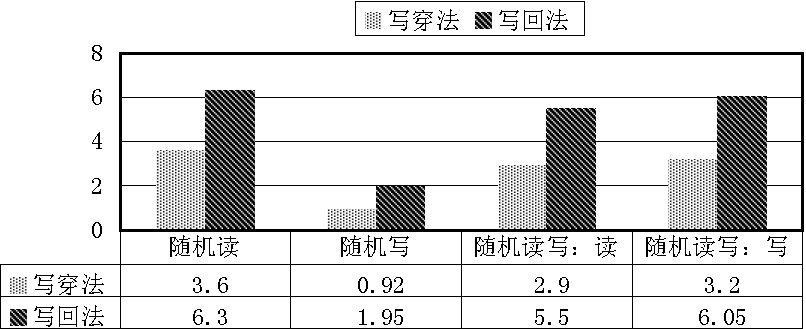
\includegraphics[width=0.9\linewidth]{./graph/enhance-rate}
\caption{读写性能提升比例比较}
\label{fig:enhance-rate}
\end{figure}

从图\ref{fig:enhance-rate}可以看出,缓存系统的存在从一定程度带来了HDD随机读、随机写的性能提升。相较于写穿法,写回法对存储系统的读写性能提升比例更为明显。

\subsection{与商业软件比较}

FancyCache是一款使用SSD作为缓存提升存储系统性能的商业软件。FancyCache可以将系统内存或SSD空间设置成机械硬盘的缓存。该软件的特点是,能够将从机械硬盘中读取的数据存入系统内存或闪存,使系统在下次访问该数据时可以很快从内存读取,避免再次读取速度较慢的硬盘,从而突破硬盘瓶颈,提升系统性能。FancyCache还能够通过特殊方式,识别并使用32位操作系统无法识别出的物理内存,解决32位Windows操作系统无法完全使用4G或更多内存的问题。

为了说明本论文实现的缓存系统与缓存软件FancyCache对系统性能提升的差距,在系统的实验阶段,论文还测试了使用FancyCache缓存软件时的HDD读写性能提升。由于通过上节的测试可以得出本论文实现的缓存系统运行于回写模式时,对HDD的随机读写性能提升最为明显。且FancyCache的软件缓存同样运行于写回模式。因此,本节会使用运行于写回模式时的测试数据与FancyCache软件进行比较。

\begin{table}[H]
\centering
\caption{随机读速度比较(KB/s)}
\begin{tabular}{|c|c|c|}
\hline
\diagbox{块大小(KB)}{缓存系统} & 本论文的 & FancyCache \\ 
\hline 4  & 2970 & 2508 \\ 
\hline 16 & 9821 & 10254 \\ 
\hline 64 & 32857 & 51833 \\ 
\hline 
\end{tabular} 
\label{tab:wb-rand-read-comp}
\end{table}

从随机读测试的结果可以看出,IO请求的大小为4KB时,本论文实现的缓存系统性能优于FancyCache;当IO请求比较大时,FancyCache的效果更为明显,这是因为论文实现的缓存系统的缓存块大小为4KB,读写请求大于4KB时会将一个读写请求切分为多个处理,影响了系统的性能。

\begin{table}[H]
\centering
\caption{随机写速度比较(KB/s)}
\begin{tabular}{|c|c|c|}
\hline
\diagbox{块大小(KB)}{缓存系统} & 本论文的 & FancyCache \\ 
\hline 4  & 2970 & 3021 \\ 
\hline 16 & 9821 & 9982 \\ 
\hline 64 & 32857 & 32258 \\ 
\hline 
\end{tabular} 
\label{tab:wb-rand-write-comp}
\end{table}

进行随机写测试,IO请求的大小为4KB和16KB时,FancyCache的性能优于本论文实现的缓存系统,但差距不大;IO请求的大小为64KB时,本论文实现的缓存系统性能略优于FancyCache。

%% ----------------------------------------------------------------------
%%% END OF FILE
%% ----------------------------------------------------------------------

%% ----------------------------------------------------------------------
%% START OF FILE
%% ----------------------------------------------------------------------
\chapter{总结与展望}
\label{cha:conclusions}

本论文首先介绍了固态硬盘和机械硬盘混合存储的技术背景和国内外存储设备厂商的相关研究工作,提出了利用固态硬盘空闲空间作为缓存,提升机械硬盘IO性能的解决方案。分析缓存技术的发展背景和支撑缓存系统的相关技术,分析不同类型存储介质的特点、混合存储技术的框架和缓存页面替换算法,进行论文方案可行的说明。

接下来,分析并详细介绍缓存系统实现中所用到的关键性技术,这些技术即包含学术和实践中已经成熟的技术:例如Windows系统的IO捕获、缓存映射策略;也包括论文提出的新技术解决方案:一种同时考虑缓存块最近最近访问时间和访问频率的缓存页面替换算法。

最后,论文给出了缓存系统的核心实现细节和性能测试结果。实现细节部分的介绍包含了缓存系统的整体设计架构、缓存算法通用接口和用户配置工具提供的参数。测试部分比较了本缓存系统和商业软件缓存系统对机械硬盘的性能提升效果。

\section{全文总结}
\label{sec:thesis_conclusion}
本论文的主要研究成果和贡献可归纳为以下几点。
\begin{enumerate}
\item
针对目前固态硬盘的价格相对机械硬盘仍然过高,存储中心大多同时使用机械硬盘和固态硬盘进行混合存储这一现状。经过综合分析了现存在的混合存储解决方案,本论文设计了一种基于固态硬盘的机械硬盘缓存存储存储架构,将固态硬盘的空闲空间用作机械硬盘上热数据的缓存,提高存储系统的IO性能。
\item
分析使用广泛的LRU、LFU等缓存页面替换算法,研究这些算法的冷热数据识别原理和实现逻辑。提出一种综合考虑最后一次访问时间和缓存块访问频数的缓存页面替换算法。
\item
在Windows平台下的实现本论文设想的混合存储缓存系统。针对大多数混合存储系统运行于Linux平台这一现状,在Windows平台使用WDM驱动开发框架实现混合存储系统,弥补Windows平台下可用的混合存储软件不足这一现状。
\item
在实现混合存储系统提供的多种缓存页面替换算法的过程中,本论文抽象出了一套可以用于所有缓存页面替换算法的通用函数接口。这套接口既降低了论文实现缓存系统时的代码复杂度,也可以作为设计页面替换算法时的功能性指导。
\item
经测试,论文实现的缓存系统的确可以带来机械硬盘性能提升,写穿模式的随机读性能有2-4倍的提升;写回模式的随机读性能有4-6倍的提升、随机写性能有有5-6倍的提升。提升效果接近商业软件FancyCache。
\end{enumerate}

\section{研究展望}
\label{sec:thesis_expectation}
随着云端计算的普及和海量数据时代的到来,计算机对现有存储系统的容量、数据可靠性和读写性能及提出了非常高的要求。固态硬盘作为一种高性能的存储设备由此产生,然而固态硬盘的价格昂贵,使得存储中心大多同时使用机械硬盘和固态硬盘进行混合存储。混合存储系统的研究也因此得到了研究人员的重视。从系统的测试结果和实现过程中的思考可以得出,论文提出的缓存系统在性能上还有很多可以提升的空间。具体可以归纳为以下几个点。


\subsubsection{结合固态硬盘特性的性能优化}

虽然固态硬盘的读写性能都高于机械硬盘的读写性能,但是固态硬盘的写性能相对于机械硬盘的优势并没有读操作的性能那么明显,而且当固态硬盘剩余的空闲空间不多时,还有可能出现严重影响写性能Write Cliff现象。针对固态硬盘写性能不是很高这一情况,下一步工作可以优化固态硬盘的写操作,整合多个连续的写请求,减少写操作的次数,提高缓存更新和缓存页面替换算法的运行效率。

\subsubsection{面向特殊场景的混合存储系统的研究}

从宏观层面看,应用程序发起的IO请求是随机且无法预测的。但是从每个程序的角度看,发起的IO请求却是有一定规律的,例如下载程序会从文件的多个位置开始顺序写文件。而且一般来说操作系统会在每个IO请求中标记发起进程的PID。缓存系统如果能够预测出某个进程的IO请求的发起模式,就可以根据模式调整缓存策略,提升系统的运行效率。因此,能够感知特殊IO请求的混合存储系统是一个新的有意义的方向。

\subsubsection{使用实时压缩算法提高缓存的空间利用率}

近几年来出现了许多优秀的用于工程实践的实时压缩算法,这类算法的压缩率虽然和主流的ZIP、RAR等软件存在差距,但是单线程的压缩速度却可以达到400MB/s以上,解压速度甚至能够达到1800MB/s。将实时压缩算法用于缓存系统,压缩率只要能够达到50\%,就可以节省一半的缓存空间。节约下来的缓存空间还可继续用于缓存数据,缓存系统命中率也会随之提高。Linux内核已使用zswap模块实时压缩交换到磁盘上的内存页面,相信这类压缩算法在缓存系统上的应用也将会得到普及。

%% ----------------------------------------------------------------------
%%% END OF FILE 
%% ----------------------------------------------------------------------


%%%%%%%%%%%%%%%
%% 论文后置部分
%%%%%%%%%%%%%%%
\backmatter

% 参考文献
\bibliographystyle{IEEEtran}
\bibliography{IEEEabrv,refs}

\iftoggle{lookuprepeat}{
}{
% 使用自定义参考文献样式,而非bibtex
\begin{thebibliography}

\bibitem{matthews2008intelturbomem}
Matthews J, Trika S, Hensgen D, Coulson R, Grimsrud K. Intel Turbo Memory: Nonvolatile disk caches in the storage hierarchy of mainstream computer systems. ACM Trans on Storage, 2008, Article 4, 24 pages.

\bibitem{jimgray2003cloud}
Jim Gray. What next?: A dozen information-technology research goals. Journal of the ACM, 2003, 50: 41–57. Turing Award lecture.

\bibitem{morris2003evostorage}
R.J.T.Morris, B.J.Truskowski. The evolution of storage. IBM SYSTEMS JOURNAL, 2003, Vol.42, No.2.

\bibitem{libo2010cacheforssd}
Li Bo, Xie Changsheng, Wang Fen, Zhao Xiaogang. New Cache Replacement Algorithm for Solid-state Drive. Computer Science, 2010, Vol.37, No.8.

\bibitem{henry2014ssdprice}
Henry Newman. SSD vs HDD Pricing: Seven Myths That Need Correcting. Enterprise Storage Forum, 2014.

\bibitem{taeho2006flashcache}
Taeho Kgil, Trevor Mudge. FlashCache: A NAND Flash Memory File Cache for Low Power Web Servers. Advanced Computer Architecture Laboratory, CASES’06, October 23–25, 2006.

\bibitem{vfcache}
中国电子科技集团公司第五十四研究所. LSI PCIe闪存适配器助力Cisco和EMC实现应用加速. 计算机与网络, 2012, 38(11).

\bibitem{smartcache}
李霁蓉. SmartCache技术在校园视频监控系统中的应用. 消费电子, 2013, 18:13-14.

\bibitem{lsiraidcache}
张明. LSI推出MegaRAID CacheCade Pro 2.0 SSD高速缓存软件. 电子工业出版社, 电子与电脑, 2011, 9:90.

\bibitem{enhanceio}
Michael Larabel. EnhanceIO: New Solid State Drive Caching For Linux. Phoronix Premium, 13 January 2013.

\bibitem{fusionio}
王珩. Fusion-io实现每秒12GB视觉特效数据传输. 计算机与网络, 2013, 16:58-58.

\bibitem{hdd2009}
Y. Shiroishi, K. Fukuda, I. Tagawa, H. Iwasaki, S. Takenoiri, H. Tanaka, H. Mutoh, N. Yoshikawa. Future Options for HDD Storage. IEEE Transactions on Magnetics, 2009, Vol 45, Issue 10.

\bibitem{ssd2009}
王伟能, 王鹤群. 固态硬盘概述. 记录媒体技术, 2009, Vol 1.

\bibitem{cache2011}
汪小林, 赖荣凤, 王振林, 罗英伟, 李晓明. 基于SSD高速缓存的桌面虚拟机交互性能优化方法. 计算机应用与软件, 2011, Vol 28, No 11.

\bibitem{zhuqing2013hybrid}
Zhu Qing, Li Xiaoyong. A Review on Hybrid Storage. Microcomputer Application, 2013, Vol.29, No.2:33-38.

\bibitem{sdramcache2002}
苏海冰, 吴钦章. 用SDRAM在高速数据采集和存储系统中实现海量缓存. 光学和精密工程, 2002, Vol 10, No 5.

\bibitem{nvramcache2013}
Sheng Qiu, A. L. Narasimha Reddy. NVMFS: A Hybrid File System for Improving Random Write in NAND-flash SSD. IEEE 29th Symposium on Mass Storage Systems and Technologies (MSST). 2013.

\bibitem{linlin2011}
Lin Lin, Yifeng Zhu, JianhuiYue, Zhao Cai, Bruce Segee. Hot Random Off-loading: A Hybrid Storage System With Dynamic Data Migration. IEEE 19th International Symposium on Modeling, 2011, Analysis Simulation of Computer and Telecommunication Systems (MAS-COTS).

\bibitem{wudong2013raid1}
Wu Dong. A Research of RAID1 Technology Based on SSD Cache. Thesis for the Degree of Master of Engineering. 2013. 1-54.

\bibitem{zhuqing2012hybrid}
Zhu Qing. Study on Hybrid Storage Systems. Thesis for the Degree of Master of Engineering. 2012. 1-56.

\bibitem{nvramcache1992}
Mary Baker, Satoshi Asami, Etienne Deprit, John Ousterhout, and Margo Seltzer. Non-volatile memory for fast, reliable file systems. International Conference on Architectural Support for Programming Languages and Operating Systems (ASPLOS), October 1992, pages 10–22, Boston, MA.

\bibitem{wdm2001}
张伟, 张云麟. Windows驱动程序模型的设计与开发. 重庆邮电学院学报:自然科学版, 2001, 第3期 88-91.

\bibitem{filterdrv2004}
梁德祥. 利用过滤层驱动程序实现移动硬盘加密. 盐城工学院学报(自然科学版), 2004, Vol 17, No 3.

\bibitem{LRU}
Marek Chrobak, John Noga. LRU is Better than FIFO. Proceedings of the ninth annual ACM-SIAM symposium on Discrete algorithms, 1998.

\bibitem{LFU}
黄秀荪, 仇玉林, 叶青. LFU算法的ASIC实现. 电子器件, 2007, 第1期, 237-240.

\bibitem{cachemap2013}
沈秀红. 基于基地址寄存器映射的数据高速缓存设计研究. 浙江大学集成电路工程硕士学位论文. 2013.

\bibitem{bplustree2012}
长孙妮妮, 张毅坤, 华灯鑫, 邹子夏, 陈浩. 一种基于B+树的混合索引结构. 计算机工程, 2012, Vol 38, No 14.

\bibitem{writeback2014}
吴纪锋, 吴文江, 秦承刚. 基于页面优先级策略的文件回写机制研究. 小型微型计算机系统, 2014, Vol 35, No 1.

\bibitem{writethrough2010}
梅魁志, 李国辉, 张斌. 一种面向写穿透Cache的写合并设计及验证. 西安交通大学学报, 2010, Vol 44, No 4, Apr.

\bibitem{writeback2008}
林伟, 叶笑春, 宋风龙, 张浩. 众核处理器中使用写掩码实现混合写回/写穿透策略. 计算机学报, 2008, Vol 31, No 11, Nov.

\bibitem{ssddesign2008}
Nitin Agrawal, Vijayan Prabhakaran, Ted Wobber, John D. Davis, Mark Manasse, and Rina Panigrahy. Design tradeoffs for SSD performance. USENIX Annual Technical Conference, 2008, pages 57–70, Boston, MA.

\bibitem{integssdhdd2011}
Yang Qing, Jin Ren. I-CASH: Intelligently Coupled Array of SSDs and HDDs. in: Proceeding of HPCA'11. Texas: IEEE Computer Society Press, 278-289, 2011.

\bibitem{cacheforflash2012}
Oh Y, Choi J, Lee D. Caching Less for Better Performance: Balancing Cache Size and Update Cost of Flash Memory Cache in Hybrid Storage Systems. FAST'12, San Jose: ACM Press, 313-326, 2012.

\bibitem{hystor2011}
Feng Chen, David Koufaty, Xiaodong Zhang. Hystor: Making the Best Use of Solid State Drives in High Performance Storage Systems. ICS (International Conference on Supercomputing), 22–32, 2011.

\bibitem{icash2011}
Jin Ren, Qing Yang. I-CASH: Intelligently Coupled Array of SSD and HDD. IEEE 17th International Symposium on High Performance Computer Architecture (HPCA), 2011.

\bibitem{computerarch2011}
李学干. 计算机系统结构. 西安电子科技大学出版社, ISBN: 9787560601397, 2011.

\bibitem{ARC}
Nimrod Megiddo, Dharmendra S. Modha. ARC: A Self-Tuning, Low Overhead Replacement Cache. FAST ’03: 2nd USENIX Conference on File and Storage Technologies, 2003.

\bibitem{windowsdrv2008}
张帆. Windows驱动开发技术详解. 电子工业出版社, ISBN: 9787121068461, 2008.

\bibitem{winkernprg2008}
谭文, 邵坚磊. 天书夜读-从汇编语言到Windows内核编程. 电子工业出版社, ISBN: 9787121073397, 2008.

\bibitem{softwaredbg2008}
张银奎. 软件调试. 电子工业出版社, ISBN: 9787121064074, 2008.

\bibitem{softwaredbg2013}
张银奎. 格蠹汇编-软件调试案例集锦. 电子工业出版社, ISBN: 9787121196072, 2008.

\bibitem{findbugs2012}
Tobias Klein. 捉虫日记. 人民邮电出版社, ISBN:9787115290441, 2012.

\bibitem{dbghacks2011}
吉岡弘隆, 大和一洋, 大岩尚宏, 安部東洋, 吉田俊輔. Debug Hacks: 深入调试的技术和工具. 电子工业出版社, ISBN: 9787121140488, 2011.

\bibitem{deepinlinux2010}
Wolfgang Mauerer. 深入Linux内核架构. 人民邮电出版社, ISBN:9787115227430, 2010.

\end{thebibliography}

}
% 附录,建议放在参考文献之后,致谢与成果部分之前
% \begin{appendix}
%   %% ----------------------------------------------------------------------
%% START OF FILE
%% ----------------------------------------------------------------------
%% 
%% Filename: appendix01.tex
%% Author: Fred Qi
%% Created: 2013-01-18 20:20:46(+0800)
%% 
%% ----------------------------------------------------------------------
%%% CHANGE LOG
%% ----------------------------------------------------------------------
%% Last-Updated: 2013-01-19 10:25:52(+0800) [by Fred Qi]
%%     Update #: 10
%% ----------------------------------------------------------------------


\chapter{公式推导}

\section{一些常用公式}
\label{sec:someeq}

$$ c^{2} = a^{2} + b^{2} $$

\section{一些重要公式}
\label{sec:importanteq}

$$ E=mc^{2}$$

$$ e^{i\theta} = \frac{cos\theta + i \sin\theta}{2} $$


%% ----------------------------------------------------------------------
%%% END OF FILE 
%% ----------------------------------------------------------------------
% \end{appendix}
\iftoggle{blindreview}{
}{
    %% ----------------------------------------------------------------------
%% START OF FILE
%% ----------------------------------------------------------------------

\begin{acknowledgments}

研究生的毕业设计论文部分暂告收尾,这同时意味着我在西安电子科技大学研究生两年半的生活将要结束。回顾两年半来在西电的学习和生活,我深深感到自己不再是像本科期间那样只是机械的上课和学习新的理论知识,而是逐渐培养了自己独立进行科研和组织、管理技术项目的能力。可以将自己最宝贵的青春时光在西电绿树成荫、风景秀美的校园中,能在众多学富五车、才华横溢的老师们的熏陶下度过,实在是荣幸至极。

在进行毕业设计的实验和毕业论文的撰写期间,正是由于导师的谆谆教诲和同学们的出谋划策才使得我克服了一个又一个的难题,他们的鼓励和支持是我完成毕业设计和毕业论文的动力源泉。在此我还要特别感谢刘凯导师,他从论文的选题、文献的采集、系统框架的设计、实验的验证、文档结构的布局一直到论文的定稿,都无私的给予了我建议和指导,没有刘凯老师的栽培和教诲,我的毕业设计和毕业论文就不可能顺利完成。

感谢我的学长赵海星、李瑞,虽然只和他们相处了一年半的时间,但他们钻研科研、严谨治学的精神一直是我学习的楷模。还要感谢张劲同学提供的\LaTeX论文模板,使用他的论文模板使我能够专注于论文的写作而不必太过关心排版的细节。谢谢他们给予我的帮助和支持。最后,由衷地感谢我的父母十几年来为支持我的学业所付出的理解、支持和辛勤劳动。 

由于时间的仓促和本人的能力有限、经验不足,整篇文章肯定会存在尚未发现的缺点和错误。恳请阅读此篇论文的老师、同学多多予以指正。对百忙之中抽出宝贵时间对本论文进行评审的各位老师深表谢意。

\end{acknowledgments}

% ----------------------------------------------------------------------
%% END OF FILE
%% ---------------------------------------------------------------------
    %% ----------------------------------------------------------------------
%% START OF FILE
%% ----------------------------------------------------------------------

\chapter*{攻读硕士学位期间的研究成果}
\label{char:achi}

\paragraph{期刊论文}

\begin{enumerate}
\item \textbf{Jinjian Wu}, Fei Qi, and Guangming Shi. “Self-Similarity Based Structural Regularity for Just Noticeable Difference Estimation,” Journal of Visual Communication and Image Representation, 23(6): 845-852, August, 2012.(SCI)

\item ...
\end{enumerate}

\paragraph{会议论文}
\begin{enumerate}
\item \textbf{Jinjian Wu}, Fei Qi, and Guangming Shi. “Image Quality Assessment Based on Improved Structural Similarity,” PCM 2012, Singapore.(EI)

\item ...
\end{enumerate}


\paragraph{参加研究的科研项目}

\begin{itemize}
\item 
\textbf{国家863计划项目}, 无线传感器网络协同获取融合与表达, 2008.1.-2009.12. (2007AA01Z307);
\item ...
\end{itemize}

% ----------------------------------------------------------------------
%% END OF FILE 
%% ---------------------------------------------------------------------
}
\end{document}

%% ----------------------------------------------------------------------
%%% END OF FILE
%% ----------------------------------------------------------------------
